\chapter{Desarrollo del Proyecto}
En este capítulo se discute sobre el trabajo a realizado para la completitud del proyecto, así como la descripción y el \textit{post-mortem} de las diferentes actividades realizadas durante su realización.

\section{Producto propuesto}
El producto desarrollado fue un videojuego multijugador. En este los alumnos pueden aprender conceptos básicos de los lenguajes de programación, viendo los conceptos de programación estructurada, mediante acertijos que les permitan de otra manera analizar su funcionamiento. En este juego se enfocó a la enseñanza de: variables, condicionales, ciclos y funciones, tratando temas de programación estructurada, basado en el material del curso de Fundamentos de la Programación de la Universidad Autónoma de Ciudad Juárez, así como los libros Fundamentos de programación: Algoritmos, estructura de datos y objetos de Luis Joyanes Aguilar y Prelude to Programming: Concepts and design de Steward Venit y Elizabeth Drake. 
Las mecánicas del juego fueron inspiradas en el videojuego \textit{Among Us}. En este juego, un grupo de máximo 10 jugadores están juntos en una partida, hay una variedad de mapas y el punto es realizar todas las actividades que tienen asignadas para ganar. Pero del grupo de jugadores, unos cuantos son asignados como impostores y su trabajo es matar a los demás jugadores. Sin embargo, los jugadores pueden reportar muertes o sonar una alarma que les permite discutir y votar por quien es impostor, si sacan a todos los impostores, ganan los \textit{crewmates}, los jugadores no impostores.
El videojuego tendrá una duración aproximada de 20-30 minutos.

\section{Forma de validación}
Para la evaluación de la eficacia del producto creado se pidió la ayuda de varios docentes que han impartido o están actualmente impartiendo clases de Fundamentos de Programación. Esto con el fin de validar el contenido por su valor didáctico, que cumpla las demandas del curso y enseñe el tema de manera correcta.

\section{Metodología}
\begin{longtable}[c]{|m{5cm}|c|c|c|}
\caption{Calendarización de actividades del proyecto \label{table:fechas_actividades}}\\
\hline
        Tarea & Fecha Inicio & Fecha Finalización & Duración \\ \hline
        Investigación de antecedentes & 12/08/2019 & 09/09/2019 & 28 \\ \hline
        Establecimiento de objetivos del proyecto & 09/09/2019 & 20/09/2019 & 11 \\ \hline
        Desarrollo del marco referencial & 16/09/2019 & 20/09/2019 & 4 \\ \hline
        Definición del producto esperado & 23/09/2019 & 23/09/2019 & 0 \\ \hline
        Cronograma de actividades & 30/09/2019 & 04/10/2019 & 4 \\ \hline
        Metodología de desarrollo & 30/09/2019 & 04/10/2019 & 4 \\ \hline
        Entrega del borrador final & 16/10/2019 & 16/10/2019 & 0 \\ \hline
        Presentación & 17/10/2019 & 17/10/2019 & 0 \\ \hline
        Atención a las observaciones de los asesores & 28/10/2019 & 13/11/2019 & 16 \\ \hline
        Presentación del desarrollo del proyecto & 15/11/2019 & 15/11/2019 & 0 \\ \hline
        Poder unirse a un lobby & 17/12/2020 & 19/12/2020 & 2 \\ \hline
        Redacción del capítulo de desarrollo del proyecto & 17/12/2020 & 31/10/2021 & 318 \\ \hline
        Jugador puede moverse por el mapa & 02/01/2021 & 02/01/2021 & 0 \\ \hline
        Jugador puede interactuar con objetos de la escena & 03/01/2021 & 03/01/2021 & 0 \\ \hline
        Jugador puede votar por un jugador como culpable & 24/01/2021 & 02/02/2021 & 9 \\ \hline
        Jugador puede agendar reuniones & 03/02/2021 & 04/02/2021 & 1 \\ \hline
        Ocultar gente muerta & 05/02/2021 & 05/02/2021 & 0 \\ \hline
        Puzzle boilers -int & 08/02/2021 & 08/02/2021 & 0 \\ \hline
        Puzzle de variable-bool & 11/02/2021 & 11/02/2021 & 0 \\ \hline
        Puzzle auto do-while & 12/02/2021 & 12/02/2021 & 0 \\ \hline
        Puzzle variable-float & 13/02/2021 & 13/02/2021 & 0 \\ \hline
        Puzzle cuarto de lavado -for & 14/02/2021 & 14/02/2021 & 0 \\ \hline
        Puzzle zaguán- llenar cubeta -while & 15/02/2021 & 15/02/2021 & 0 \\ \hline
        Puzzle if & 16/02/2021 & 16/02/2021 & 0 \\ \hline
        Puzzle if/else & 17/02/2021 & 17/02/2021 & 0 \\ \hline
        Jugadores asesinos pueden ejecutar sabotajes & 19/02/2021 & 23/02/2021 & 4 \\ \hline
        Puzzle de saboteo de telégrafo (cuestionario) & 19/02/2021 & 25/02/2021 & 6 \\ \hline
        Puzzle para saboteo para electricidad & 19/02/2021 & 25/02/2021 & 6 \\ \hline
        Sabotajes pueden ser detenidos únicamente por junta por esqueleto encontrado & 25/02/2021 & 04/03/2021 & 7 \\ \hline
        Configurar protocolo websockets para conexión cliente/servidor & 08/03/2021 & 10/05/2021 & 63 \\ \hline
        Puzzle string & 17/03/2021 & 18/03/2021 & 1 \\ \hline
        Puzzle de secuencia & 21/03/2021 & 22/03/2021 & 1 \\ \hline
        Puzzle string-substring & 23/03/2021 & 24/03/2021 & 1 \\ \hline
        Agregar sprites terminados al juego & 25/03/2021 & 27/03/2021 & 2 \\ \hline
        Conectar a UI sistema de asesinos y programadores & 13/05/2021 & 15/05/2021 & 2 \\ \hline
        Hacer jugador transparentoso cuando haya muerto, y solo mostrar a otros jugadores muertos. Spawnear tumbita para los que esta vivos & 15/05/2021 & 16/05/2021 & 1 \\ \hline
        Pasar bandera si es asesino de la selección que ocurrió al estar todos listos en el lobby & 17/05/2021 & 18/05/2021 & 1 \\ \hline
        Agregar \textit{cooldowns} después de votación para volver a activar las juntas de emergencia y de los asesinos poder matar a los programadores & 18/05/2021 & 21/05/2021 & 3 \\ \hline
        Asignar nombre al jugador cuando no puso ninguno en el \texit{lobby} & 25/05/2021 & 26/05/2021 & 1 \\ \hline
        Actualizar \textit{sprite} del jugador a el personaje elegido en el \textit{lobby} & 27/05/2021 & 29/05/2021 & 2 \\ \hline
        Pantalla para mostrar si jugador ha ganado o perdido al final del juego & 29/05/2021 & 30/05/2021 & 1 \\ \hline
        Puzzle de saboteo para boiler & 03/06/2021 & 04/06/2021 & 1 \\ \hline
        Pantalla de elección de jugador & 13/06/2021 & 14/06/2021 & 1 \\ \hline
        Agregar información de las vueltas realizadas en puzzle for & 21/06/2021 & 22/06/2021 & 1 \\ \hline
        Crear contenedores Docker para correr el servidor y el web server & 04/07/2021 & 14/08/2021 & 41 \\ \hline
        Trabajar en sistema de votación para expulsar asesinos & 16/07/2021 & 26/07/2021 & 10 \\ \hline
        Hacer pruebas y corrección de errores antes de la verificación de requerimientos & 24/08/2021 & 30/09/2021 & 37 \\ \hline
        Cambiar puzzle string por un puzzle de rellenar ciclo para & 02/10/2021 & 03/10/2021 & 1 \\ \hline
        Redacción del capítulo 4 del documento & 04/10/2021 & 10/11/2021 & 37 \\ \hline
        Reunión con primer docente & 06/10/2021 & 06/10/2021 & 0 \\ \hline
        Rediseñar puzzles para usar sintaxis de PSeInt & 08/10/2021 & 14/10/2021 & 6 \\ \hline
        Rediseñar puzzle de int a float a integrar SiNo para hacerlos de ver resultado de pseudocódigo & 09/10/2021 & 12/10/2021 & 3 \\ \hline
        Rediseñar puzzle secuencia para definir un algoritmo para llegar al otro lado & 12/10/2021 & 18/10/2021 & 6 \\ \hline
        Rediseñar puzzle For & 14/10/2021 & 15/10/2021 & 1 \\ \hline
        Rediseñar puzle DoWhile & 14/10/2021 & 16/10/2021 & 2 \\ \hline
        Rediseñar puzzle Bool a ser de seleccionar que hace el seudocódigo & 15/10/2021 & 16/10/2021 & 1 \\ \hline
        Agregar ayudas para si se atoran los jugadores & 16/10/2021 & 19/10/2021 & 3 \\ \hline
        Hacer que sprite el jugador se voltee a la dirección de movimiento & 18/10/2021 & 18/10/2021 & 0 \\ \hline
        Corregir errores en seudocódigo de ejercicios & 22/10/2021 & 26/10/2021 & 4 \\ \hline
        Cambiar número de jugadores máximo a 25 & 23/10/2021 & 23/10/2021 & 0 \\ \hline
        Ocultar nametag de impostores en modo fantasma & 24/10/2021 & 25/10/2021 & 1 \\ \hline
        Crear documentación de instalación y funcionamiento del juego & 27/10/2021 & 03/11/2021 & 7 \\ \hline
        Redacción del capítulo 5 del documento & 31/10/2021 & 10/11/2021 & 10 \\ \hline
        Reuniones con docentes 2 y 3 & 01/11/2021 & 01/11/2021 & 0 \\ \hline
        Reuniones con docentes 3 y 4 & 03/11/2021 & 03/11/2021 & 0 \\ \hline
        Redacción de la introducción del documento y detalles finales & 04/11/2021 & 08/11/2021 & 4 \\ \hline
\end{longtable}

Kanban fue la metodología usada para el desarrollo del proyecto. Para la organización del tablero usamos una aplicación multiplataforma llamada  \textit{Notion} (figura~\ref{fig:notion_proyecto}), de la cual se aprovechó su vista de tablero Kanban, lista de actividades y diagrama de Gantt. En los siguientes puntos se presenta el plan de actividades llevadas a cabo (y su descripción con mayor detalle) en la realización del proyecto. En la tabla~\ref{table:fechas_actividades} y la figura~\ref{fig:diagrama_gantt} se puede ver las actividades realizadas a lo largo de la duración del proyecto. Desde las actividades del anteproyecto, pasando por la definición del producto esperado, hasta la realización del proyecto. 

Cómo anteriormente se había tratado, el tiempo de ciclo o \textit{Lead Time} es el tiempo de realización de la tarea, abarca desde que se empieza a trabajar hasta que se completa la tarea. Por lo general, es bueno cuando el tiempo de ciclo es corto porque significa que no hay obstáculos que el equipo de trabajo tenga que resolver. De manera similar, como se nota en la figura~\ref{fig:grafica_tiempos_ciclo} y en la figura~\ref{fig:grafica_flujo_acumulado} la mayoría de las actividades fueron resueltas en corto tiempo, la única excepción fueron actividades donde surgieron problemas técnicos no esperados, los \textit{unknown unknowns}. El principal motivo de estos fue el uso de la librería \textit{Mirror} que aumento la complejidad por la sincronización entre el cliente y la documentación de la librería es muy escasa arriba de la configuración básica, incluso considerando la de su predecesora, Unet.

\begin{figure}[H]
    \centering
    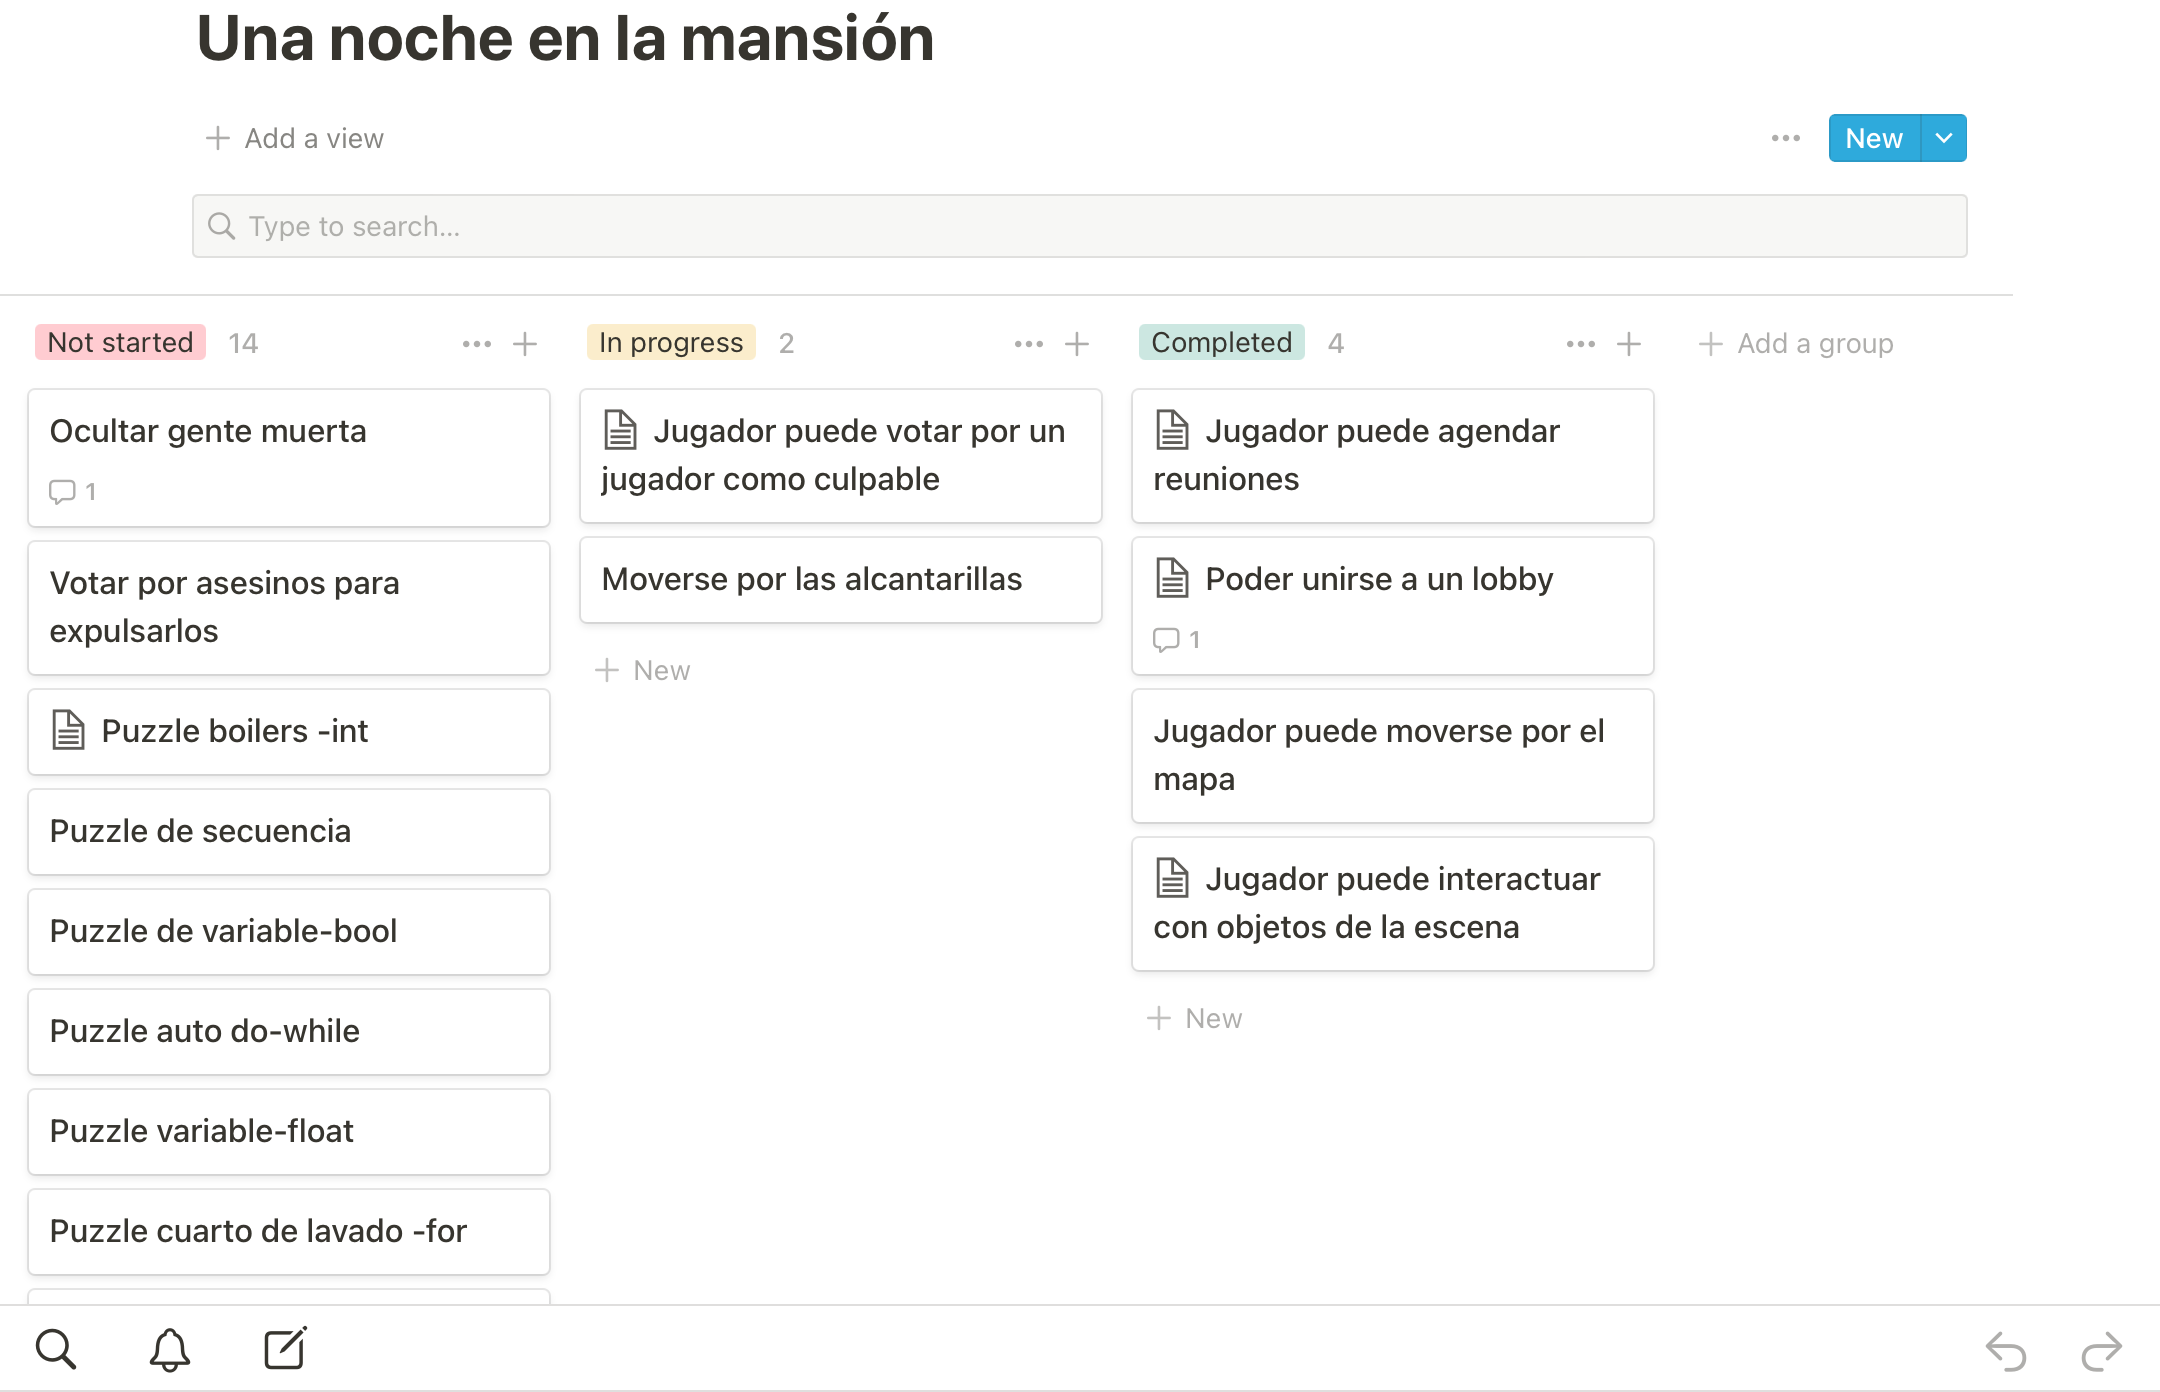
\includegraphics[width=0.8\linewidth]{images/notion.png}
    \caption{Notion con las actividades en diagrama \textit{Kanban}}
    \label{fig:notion_proyecto}
\end{figure}
\begin{figure}
    \centering
    \caption{Diagrama de Gantt del proyecto}
    \label{fig:diagrama_gantt}
    \begin{subfigure}{\textwidth}
        \centering
        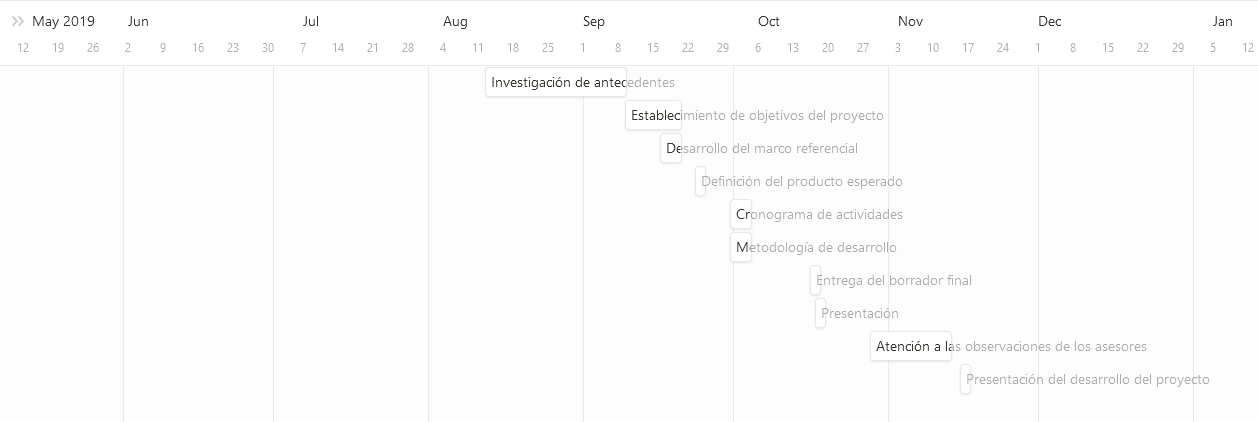
\includegraphics[width=0.8\linewidth]{images/ago-dec-19.png}
        \caption{Diagrama de Gantt del anteproyecto}
        \label{fig:gantt_anteproyecto}
    \end{subfigure}
    \begin{subfigure}{\textwidth}
        \centering
        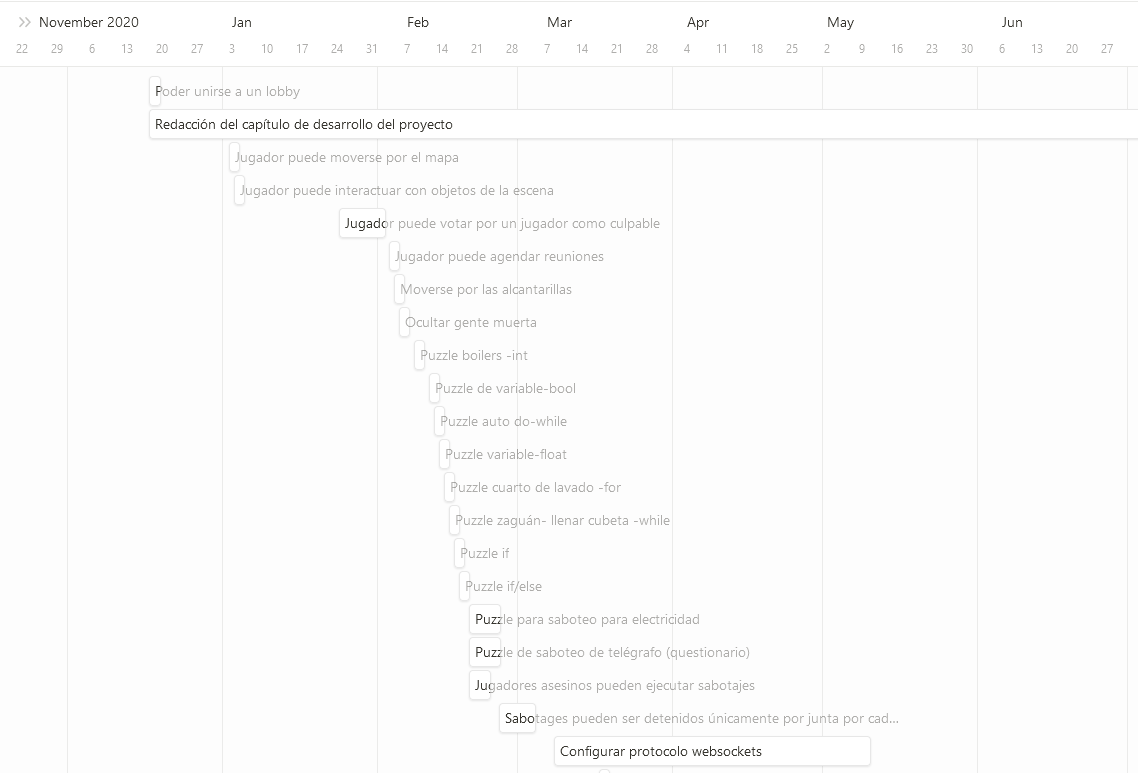
\includegraphics[width=0.8\linewidth]{images/ene-mar-21.png}
        \caption{Diagrama de Gantt de la realización del proyecto - Noviembre 2020 a Marzo 2021}
        \label{fig:gantt_proyecto}
    \end{subfigure}
\end{figure}
\begin{figure}
    \ContinuedFloat
    \centering
    \caption{Diagrama de Gantt del proyecto}
    \label{fig:diagrama_gantt}
         \begin{subfigure}{\textwidth}
        \centering
        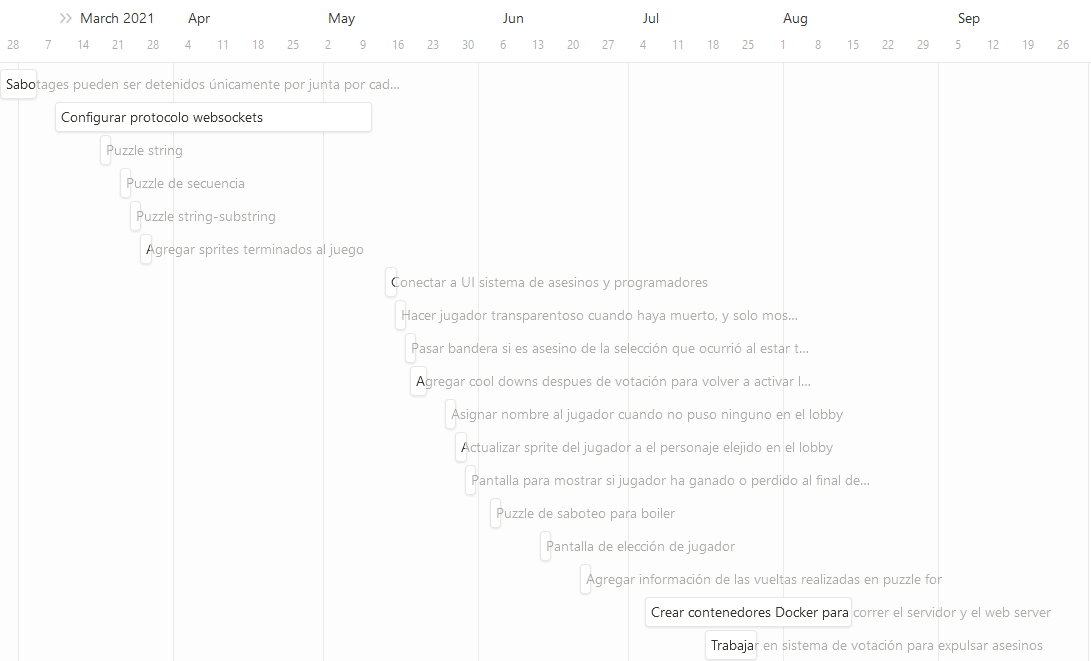
\includegraphics[width=0.8\linewidth]{images/mar-sep-21.png}
        \caption{Diagrama de Gantt de la realización del proyecto - Marzo 2021 a Septiembre 2021}
        \label{fig:gantt_proyecto_2}
    \end{subfigure}
    \begin{subfigure}{\textwidth}\ContinuedFloat
        \centering
        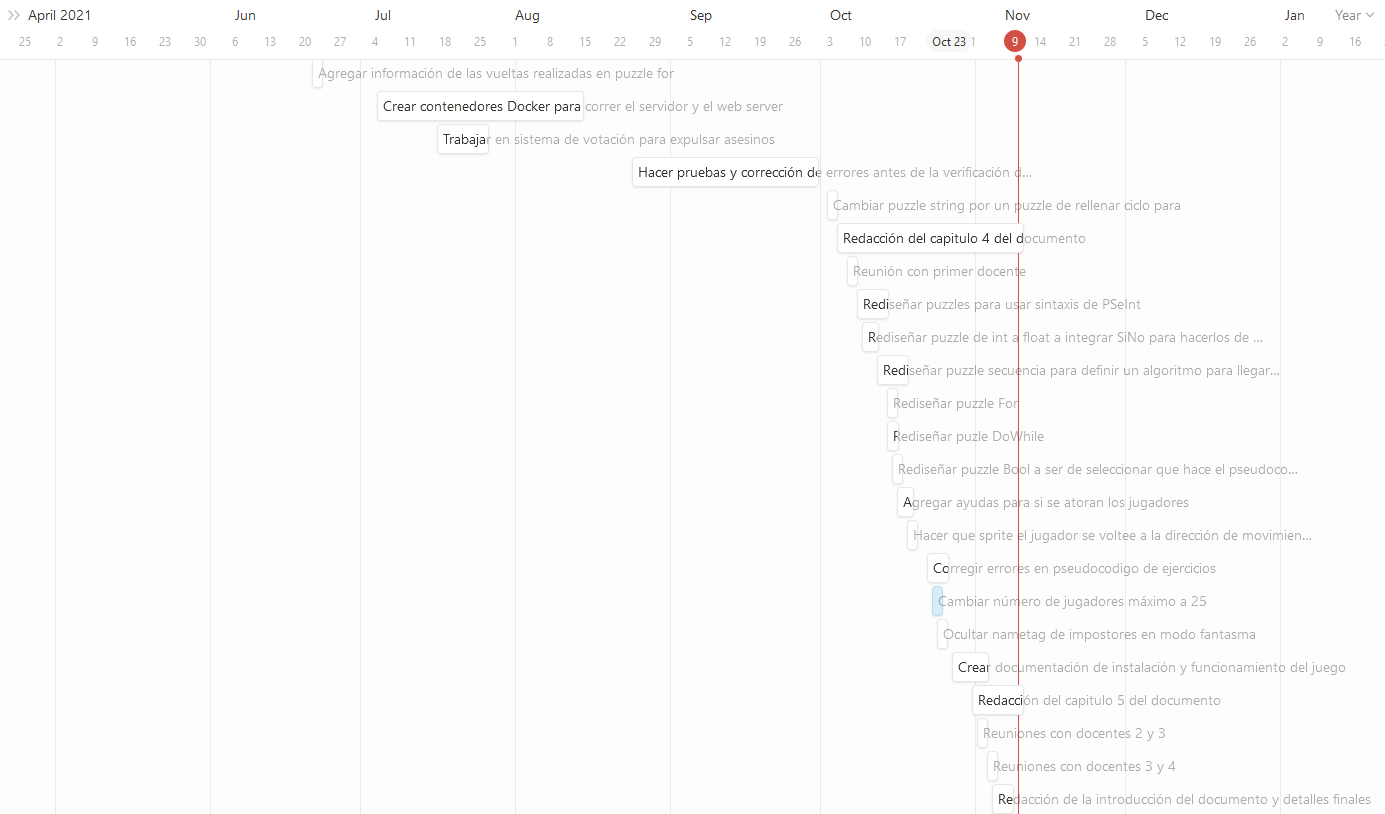
\includegraphics[width=0.8\linewidth]{images/sep-nov-21.png}
        \caption{Diagrama de Gantt de la realización del proyecto - Septiembre 2021 a Noviembre 2021}
        \label{fig:gantt_proyecto_3}
     \end{subfigure}
\end{figure}
\begin{figure}[H]
    \centering
    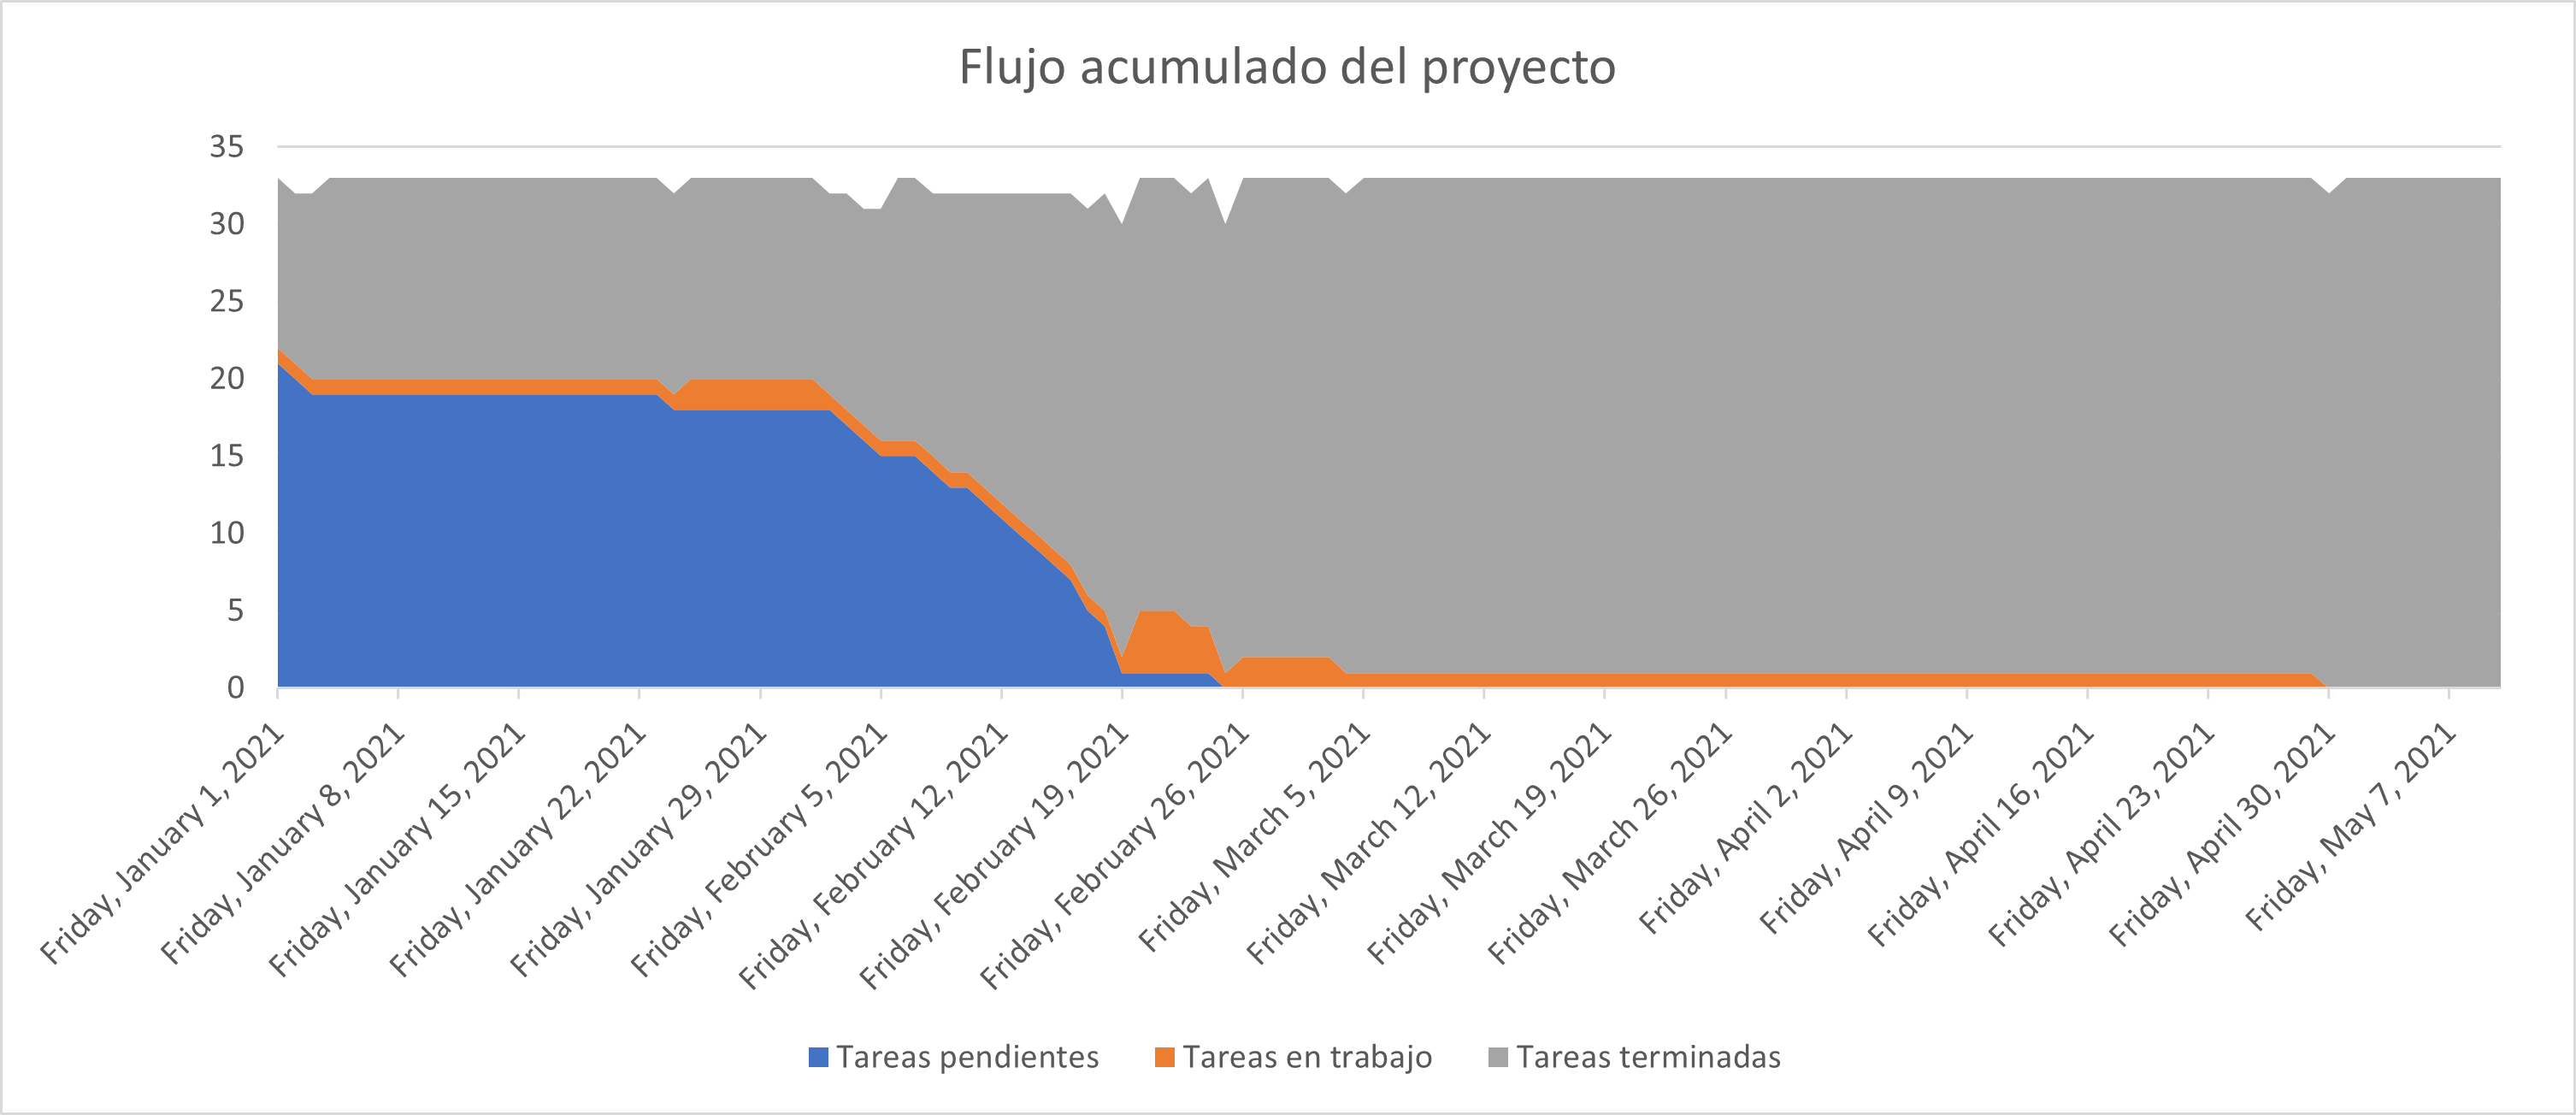
\includegraphics[width=0.8\linewidth]{images/BurndownChart.png}
    \caption{Gráfica de flujo acumulado del proyecto}
    \label{fig:grafica_flujo_acumulado}
\end{figure}
\begin{figure}[H]
    \centering
    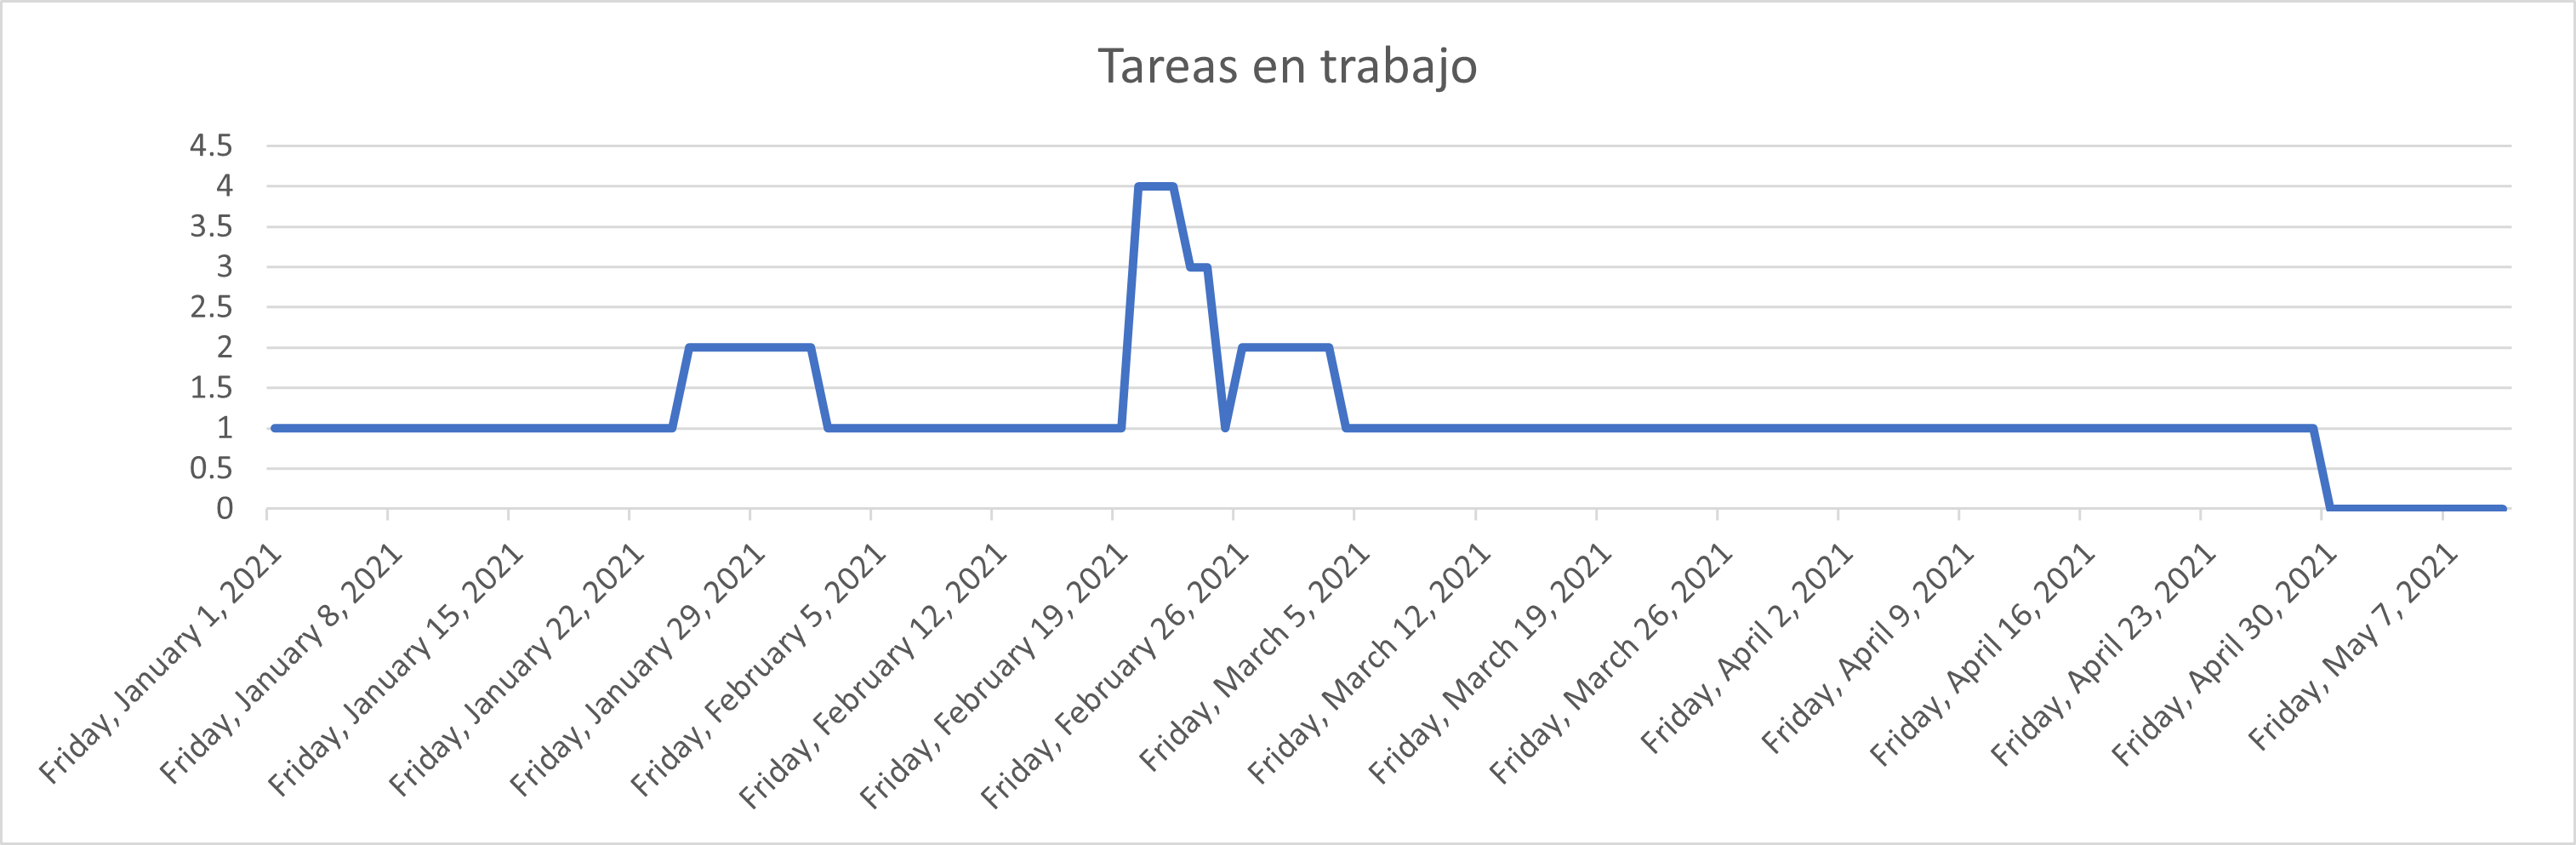
\includegraphics[width=0.8\linewidth]{images/TareasEnTrabajo.png}
    \caption{Gráfica de distribución de tiempos de ciclo del proyecto}
    \label{fig:grafica_tiempos_ciclo}
\end{figure}

\subsection{Análisis}
\subsubsection{Propuestas de producto}
Durante la definición del proyecto empezó la pandemia del SARS-COV2 que genera el padecimiento COVID-19. Ante la necesidad del aislamiento mucha gente recurrió a una gran variedad de juegos para ocupar su tiempo libre, entre estos hubo algunos juegos que ocuparon la consciencia colectiva por al menos un rato, juegos como \textit{Animal Crossing}, \textit{Fall Guys} y \textit{Among Us}. Muchos de estos juegos la gente los descubrió en \textit{streams}(transmitido en tiempo real) de gente jugando con sus amigos, estos normalmente jugaban el juego mientras estaban en videollamada. Un juego con ventajas similares que funcione tanto en un entorno en línea, así como en un salón de clases, tiene la utilidad como actividad integradora porque naturalmente hace que entre compañeros hablen y permite conocer a otras personas.
En su parte, se enfocó a que la creación del juego el usuario pueda aprender programación junto con sus compañeros incluso cuando estos no comparten un mismo espacio físico, dado que, durante la definición de este, muchos estudiantes tuvieron la necesidad de tomar clases a distancia. Ante esto, la preferencia que el juego fuera accesible en una multitud de dispositivos, a fin de que una gran variedad de estudiantes pueda acceder con su dispositivo o un dispositivo de la institución para participar en la actividad. Con este factor se consideró la necesidad de crear un juego para navegador como producto final. A base de la experiencia previa, así como sus plataformas soportadas y su facilidad para el desarrollo se decidió usar \textit{Unity} como \textit{game engine}.

\section{Diseño}
\subsection{Documento de diseño}
Se trabajó en un documento detallando los diferentes sistemas del juego. En este se definieron aspectos del juego como los diferentes puzzles como ejercicios de programación que tendrá que realizar el jugador para avanzar en el juego, el arte del juego, habitaciones, mecánicas, etc.

\subsubsection{Puzzles}
Los puzzles del juego fueron pensados para traer analogías del mundo real para explicar el funcionamiento de los diferentes conceptos a tratar. Con la limitante que el juego está orientado en Inglaterra en la tarde época victoriana, cuando invenciones como la electricidad empezaron a ganar fuerza.
Para cubrir los conceptos de programación estructurada se crearon los siguientes \textit{puzzles}:

\begin{itemize}
    \item Secuencia: Entrena al jugador en lógica de programación al trabajar en este la habilidad de resolver problemas paso a paso. En este \textit{puzzle} el jugador tiene que crear el algoritmo con los pasos necesarios para hacer que el robot llegue de un lado al otro (figura~\ref{fig:puzzle_secuencia}).
    \begin{figure}[H]
        \centering
        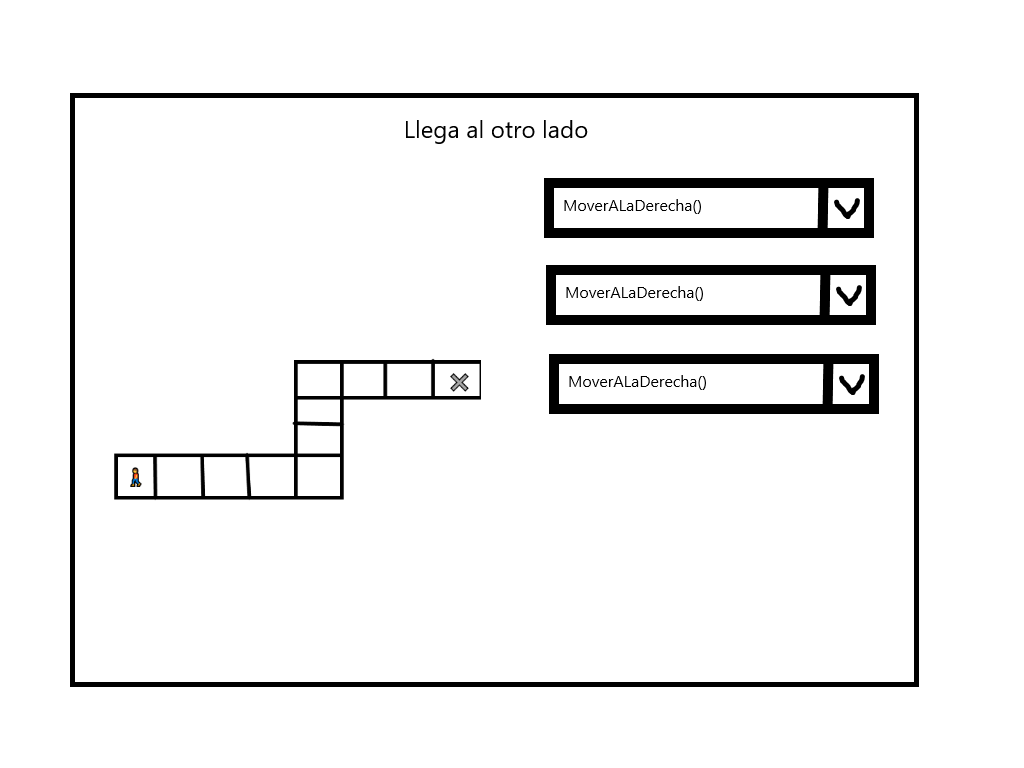
\includegraphics[width=0.5\linewidth]{images/PuzzleSecuencia.png}
        \caption{Prototipo del puzzle de secuencias}
        \label{fig:puzzle_secuencia}
    \end{figure}
    \item Ciclos
    \begin{itemize}
        \item Opción múltiple: En este tipo de \textit{puzzle}, se pide al jugador que seleccione el ciclo con un numero definido de repeticiones. Dependiendo de la dificultad, puede que se combinen varios tipos de ciclos en sus opciones. 
        \item Completar ciclo: Tiene instrucciones de cuantas repeticiones debe hacer el bucle. El jugador tiene que completar el valor de pasos, de inicio de la variable de índice y cuando termina de correrse el ciclo.
    \end{itemize}
    \item Condicionales: Hay varios puzzles tratando condicionales a lo largo del juego. La formula general es que tienen que seleccionar lo que hace ese pedazo especifico de código. Un ejemplo, se puede ver en la figura~\ref{fig:if_else_puzzle}. Sin embargo, como lo hace cada uno varia ligeramente.
    \begin{figure}[H]
                \centering
                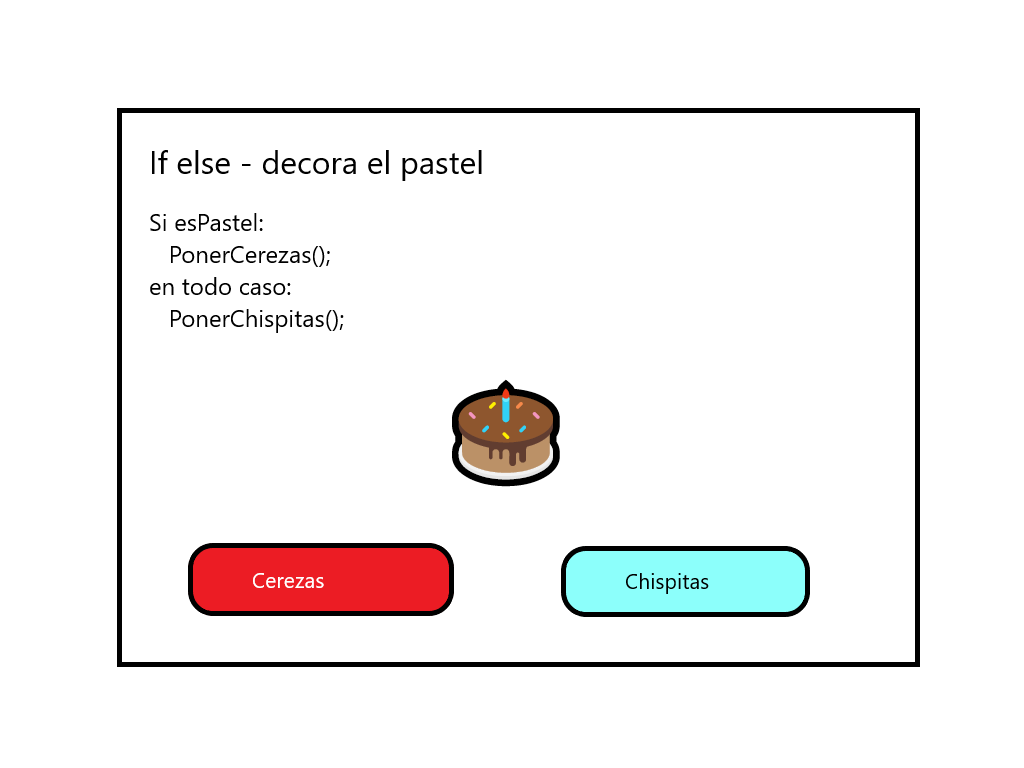
\includegraphics[width=0.5\linewidth]{images/PuzzleIfElse.png}
                \caption{Puzzle diseñado para el if/else}
                \label{fig:if_else_puzzle}
            \end{figure}
    \begin{itemize}
        \item If: El jugador tiene que razonar el pseudocódigo dado y ver si la condición ambos tipos de flores son iguales ocurre. Dependiendo de eso que rama va agarrar el programa y como impacta eso a lo que realiza este.
        \item If/else: El usuario lee un pedazo de pseudocódigo, lo analiza para ver que hace, y elige la opción que marca lo que hizo el código. El pedazo dice como se va a decorar un pastel, el usuario tiene que analizar el código y decir si se va a decorar con cerezas o con chispitas.
    \end{itemize}
\end{itemize}

Es importante destacar que estos son los \textit{puzzles} finales, algunos se han cortado del juego o modificado. Esto se discutirá en mas detalle en el capitulo próximo. 

La organización de los puzzles se puede ver la figura~\ref{fig:items_on_map}. La mayoría de los puzzles están organizados dependiendo en su temática, por ejemplo: decoración de pasteles ocurre en la cocina. Sin embargo, se tomaron a la hora del diseño libertades para hacer que cuartos sean más justos, hay puzzles que su posición fue definida para crear un flujo de jugadores en ese cuarto, a forma de que haya lugares donde los asesinos pueden ir varias veces a encontrar jugadores programadores y a la vez evitar que si los agarran en estos lugares nadie se dé cuenta.
Los \textit{puzzles} se pueden descubrir por un símbolo de espada (figura~\ref{fig:puzzle_location}), los jugadores se tienen que parar cerca para interactuar con ellos, eso abre la interfaz gráfica para resolver los puzzles. Cuando estos no hayan sido resueltos tienen un icono, cuando ya fueron resueltos por un jugador este desaparece y no se puede interactuar con ellos.

\begin{figure}[H]
    \centering
    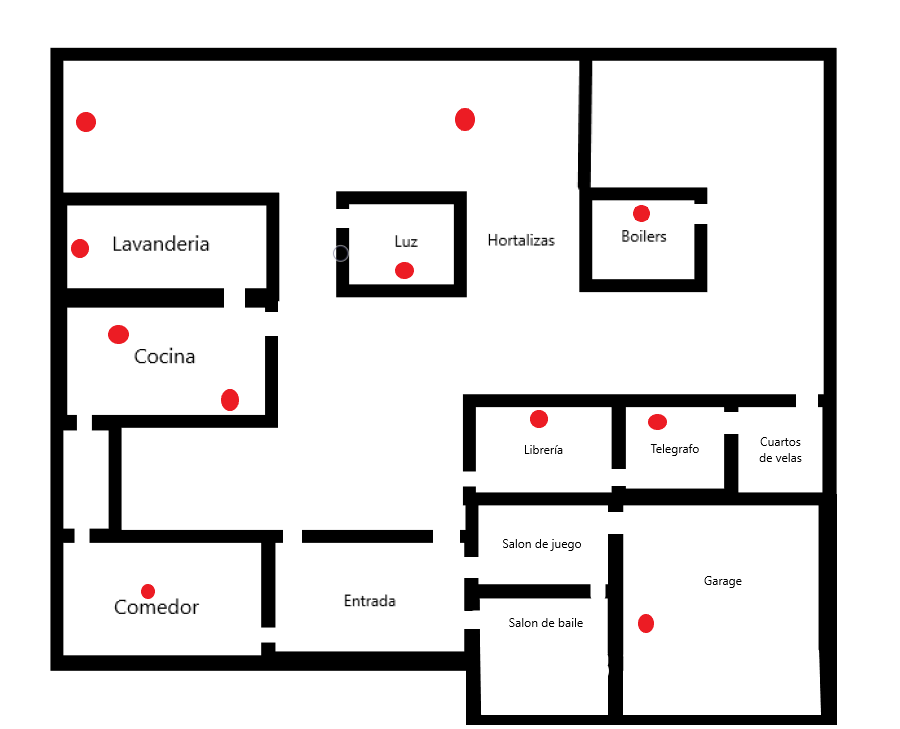
\includegraphics[width=0.5\linewidth]{images/MapaJuegoConItems.png}
    \caption{Disposición de \textit{puzzles} en el juego}
    \label{fig:items_on_map}
\end{figure}

\begin{figure}[H]
    \centering
    
\includegraphics[scale=0.5]{images/espada_sprite.png}
    \caption{\textit{Sprite} que indica que en ese lugar del juego es un \textit{puzzle}}
    \label{fig:puzzle_location}
\end{figure}

\begin{figure}[H]
    \centering
    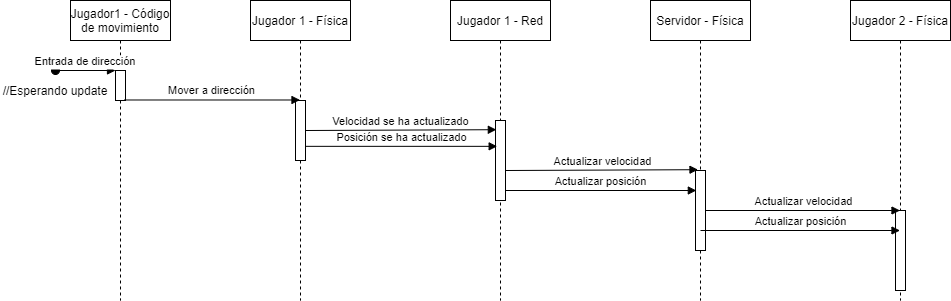
\includegraphics[width=1\linewidth]{images/diagrama_secuencia_movimientos.png}
    \caption{Diagrama de secuencia de los controles del jugador}
    \label{fig:diagrama_sec_movimiento}
\end{figure}

Se decidió utilizar la librería \textit{Mirror} para desarrollar el sistema de multijugador. Esto es esencial, porque sus abstracciones para el manejo de las comunicaciones cliente-servidor mediante \textit{Remote Call Procedure} dictaron algunas decisiones de arquitectura.
Este fue diseñado con un servidor autoritativo. Las acciones del jugador van al servidor para ser verificadas. Una excepción es el sistema de movimiento de los jugadores, como trataremos a continuación. Como se puede ver en la figura~\ref{fig:diagrama_sec_movimiento}, en este caso cada "propietario" de su personaje tiene capacidad total de moverlo a donde quiera, en teoría. En práctica, el cliente controla la posición a base de la entrada del jugador y usando sincronización de posición y velocidad de Mirror tenemos un pseudo sistema de predicción de su siguiente movimiento para conexiones lentas. 

\subsubsection{Sistema de detección de muertes}
Es un sistema que funciona primordialmente en el servidor, se puede notar su funcionamiento en la figura~\ref{fig:diagrama_sec_detect_muertes}. En todo momento, cada \textit{game loop} corre una rutina que realiza \textit{raytracing} al área circundante al jugador con un radio definido previamente en el \textit{lobby} del juego. Al haber un cambio se mandará una llamada a un procedimiento en el cliente que actualizará la interfaz gráfica para mostrar un botón de reportar muertos. Una vez al ser reportado, se realizará una segunda revisión de que sea una operación legal y se pide a todos los clientes mostrar una UI para realizar la votación sobre el personaje de juego.
\begin{figure}[h!]
    \centering
    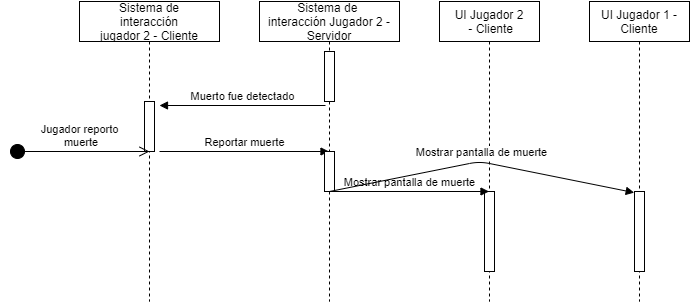
\includegraphics[width=1\linewidth]{images/diagrama_deteccion_muerte.png}
    \caption{Diagrama de secuencia de la detección de muertes}
    \label{fig:diagrama_sec_detect_muertes}
\end{figure}

\subsubsection{Asesinatos}
\begin{figure}[H]
    \centering
    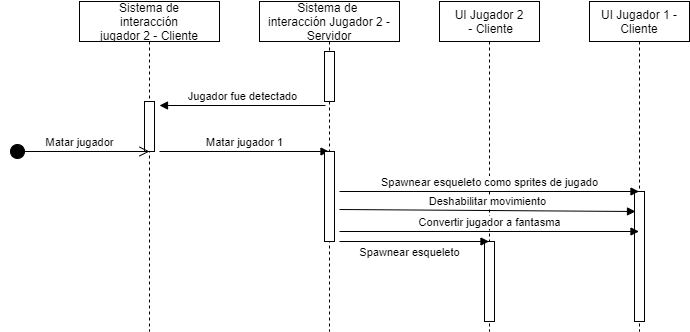
\includegraphics[width=1\linewidth]{images/diagrama_sec_matar.png}
    \caption{Diagrama de secuencia de muertes por asesinos/impostores}
    \label{fig:diagrama_sec_muertes_por_impost}
\end{figure}
Hay un tipo de jugadores especiales llamados asesinos, estos son impostores que engañan a los demás jugadores de su verdadera identidad. Estos tienen entre una de sus capacidades matar a otros jugadores. El asesinar a otros jugadores es una actividad que solo el servidor tiene autoridad.
Como se nota en la figura~\ref{fig:diagrama_sec_muertes_por_impost}, se detectan los jugadores en el servidor. En el cliente del jugador impostor se puede matar a otros jugadores no impostores, cuando se manda la señal de matar a alguien (invocada por un botón) se pregunta al servidor si es legal o sea si es físicamente posible su ocurrencia (cercanía, no hay \textit{cooldown}, entre otros). Si es legal (si en ese momento puede matar a otro jugador), se llama el \textit{spawn} de una tumba en el lugar del jugador muerto y para mandarlo a otro \textit{layer} que no es visible a los jugadores vivos y mostrar la capa de fantasmas en la cámara del cliente para el jugador muerto mediante una función RPC. En el caso de los demás jugadores solo recibirán por parte del servidor un mensaje para \textit{spawnear} una tumba y desaparecerá ese jugador de su juego.

\subsubsection{Votación de asesinos}
La votación se puede invocar de dos formas distintas; la primera forma es cuando algún jugador (ya sea programador o asesino) reporta que encontró una tumba y la segunda es acudiendo a el botón de emergencia ubicado cerca del punto donde los jugadores inician la partida. Cuando la votación se muestra una UI que permite votar por quien es el impostor (figura~\ref{fig:diagrama_ui_votacion}). En esta parte, los jugadores pueden hablar (en su salón de clases, en videollamada o \textit{chat} de voz usando una aplicación externa) para llegar a un acuerdo por quién votar, puede compartir información o pistas que encontraron durante su partida, decir que tareas tuvieron antes de la votación, etc. La votación ocurre con un tiempo límite definido, al acabarse se contabilizan los votos recibidos, en este caso pueden ocurrir tres escenarios:
\begin{itemize}
    \item Un jugador tiene la mayoría de los votos, se mata tal jugador
    \item Dos o más jugadores tienen la misma cantidad de votos, no se elimina a nadie dado que se considera un empate
    \item La mayoría de los jugadores no votaron o decidieron no votar por nadie, abstinencia de votos, no se elimina a nadie porque no hubo un acuerdo
\end{itemize}
El flujo de la votación entre el cliente y el servidor se puede observar en la figura~\ref{fig:diagrama_sec_votacion}.

\begin{figure}[H]
    \centering
    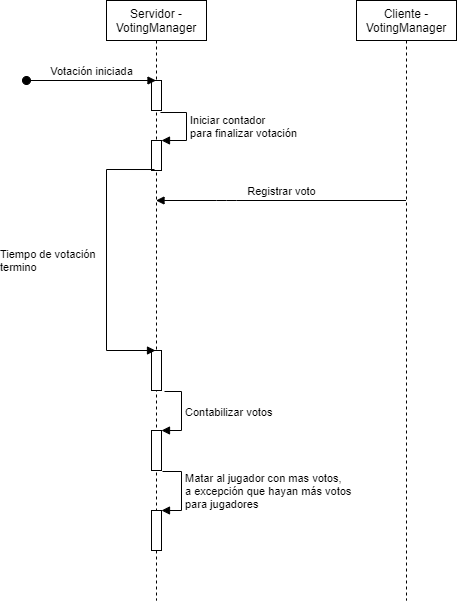
\includegraphics[width=0.5\linewidth]{images/diagrama_secuencia_votos.png}
    \caption{Diagrama de secuencia del sistema de votación}
    \label{fig:diagrama_sec_votacion}
\end{figure}
\begin{figure}[H]
    \centering
    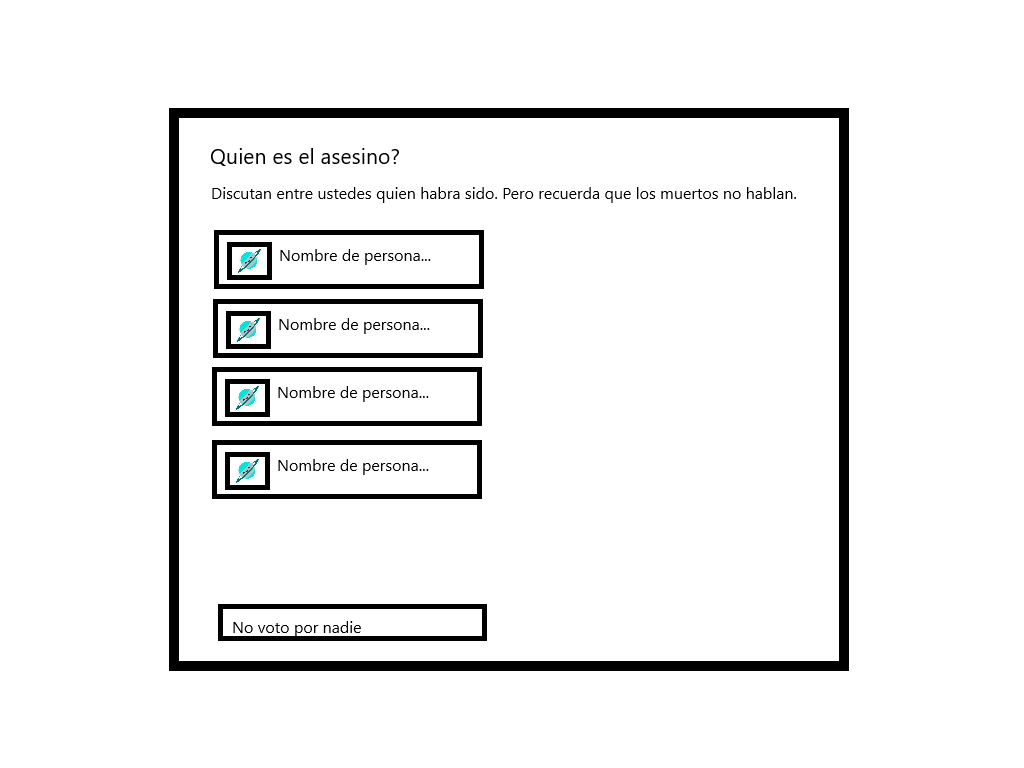
\includegraphics[width=0.5\linewidth]{images/votacion.png}
    \caption{Diseño de interfaz gráfica pantalla de votación de asesinos}
    \label{fig:diagrama_ui_votacion}
\end{figure}

\subsubsection{Modo fantasma}
Para balancear el hecho de que hay lugares de mapa donde los asesinos pueden quedarse atorados sin posibilidad de escapar después de acabar con otro jugador, se diseñó el modo fantasma. Al completar un \textit{puzzle} algún jugador como asesino se agrega una posibilidad de usar el modo fantasma que le permitirá volverse transparente y realizar una salida de estos cuartos.

\subsubsection{Emergencias}
Son tipos especiales de \textit{puzzles}. Tienen la misma complejidad que estos, pero requieren 2 jugadores que los hagan al mismo tiempo para completarlos con éxito. Estos pueden ocurrir varias veces en la partida dependiendo de los asesinos. Estos pueden invocar las emergencias después de un tiempo dado de que haya iniciado la partida, después de un tiempo de juntas y después de un tiempo de que los programadores completaron una primera emergencia correctamente.

    \begin{figure}[H]
        \centering
        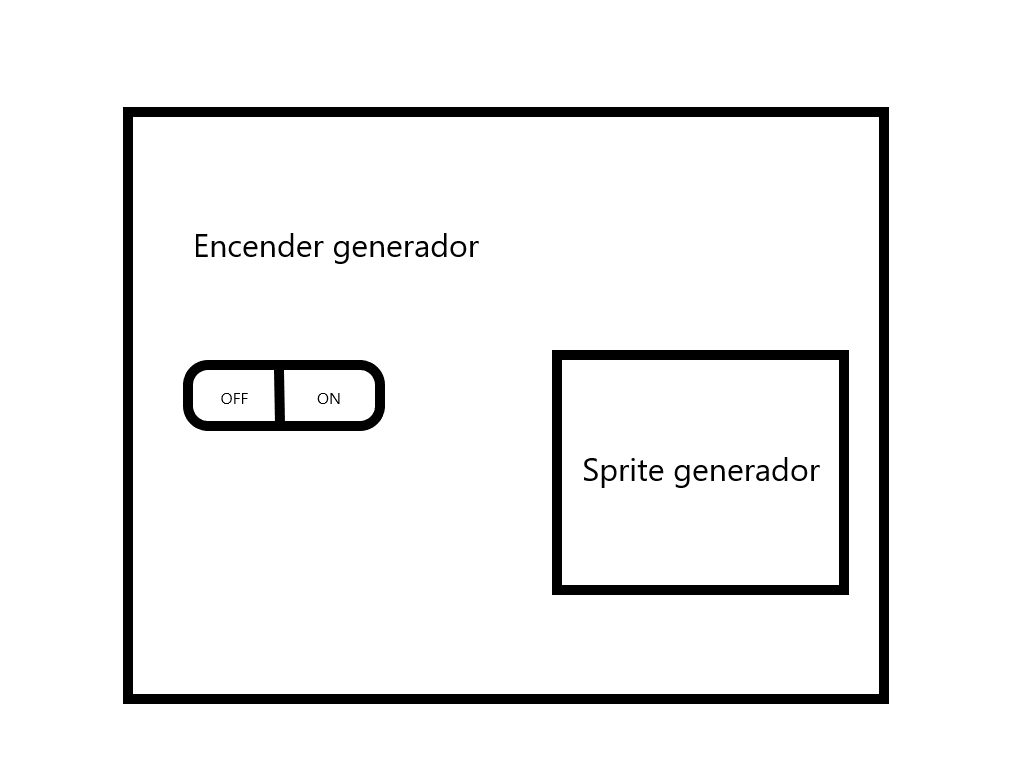
\includegraphics[width=0.5\linewidth]{images/SabotageGenerador.png}
        \caption{Interfaz gráfica de emergencia en los generadores de electricidad}
        \label{fig:ui_sab_generador}
    \end{figure}
        \begin{figure}[H]
        \centering
        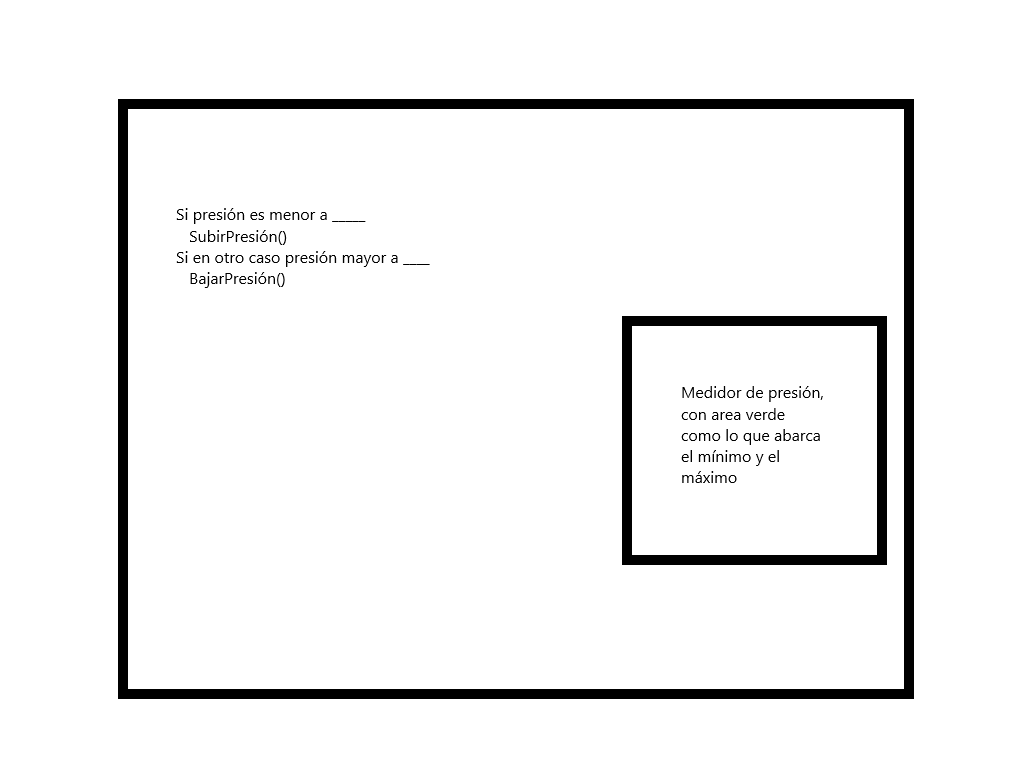
\includegraphics[width=0.5\linewidth]{images/SabotagePresion.png}
        \caption{Interfaz gráfica de emergencia en los boilers}
        \label{fig:ui_sab_presion}
    \end{figure}
        \begin{figure}[H]
        \centering
        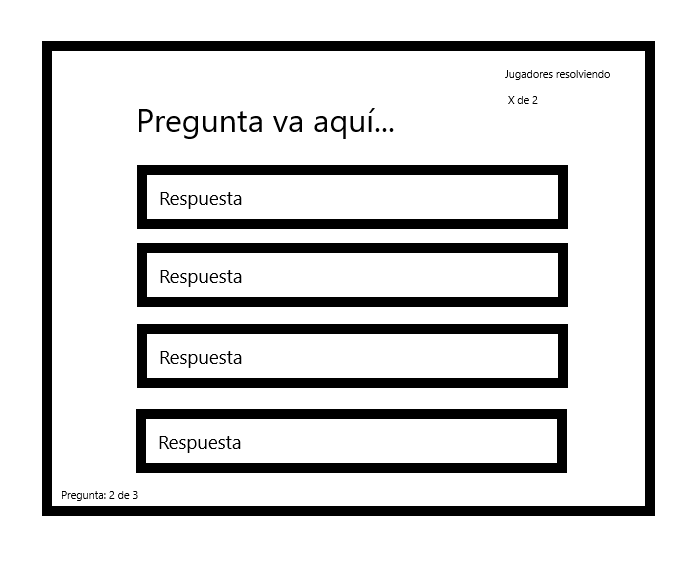
\includegraphics[width=0.5\linewidth]{images/sabotage_preguntas.png}
        \caption{Interfaz gráfica de emergencia de telégrafo}
        \label{fig:ui_teletransporte}
    \end{figure}

Hay tres emergencias disponibles:
\begin{itemize}
    \item Apagar generadores, jugadores tienen que encender un generador de respaldo. En esta emergencia los jugadores necesitan aumentar el valor de un \textit{slider}, haciendo que los jugadores experimenten con un uso potencial de las variables de números enteros (figura~\ref{fig:ui_sab_generador}).
    \item Mover presión de \textit{boilers}, jugadores tienen que regular la presión. \textit{Puzzle} consiste en que los jugadores tienen que ver el indicador en pantalla y mantener la presión en verde, modificando el algoritmo en pantalla de forma que mantenga la presión entre el mínimo y el máximo (figura~\ref{fig:ui_sab_presion}).
    \item Sabotear telégrafo, requiere dos personas contesten preguntas. Al contestar un numero de dado de preguntas correctas resolverán la emergencia. La interfaz gráfica se puede ver en la figura~\ref{fig:ui_teletransporte}.
\end{itemize}

\subsubsection{Mapa de juego}
\begin{figure}[h]
    \centering
    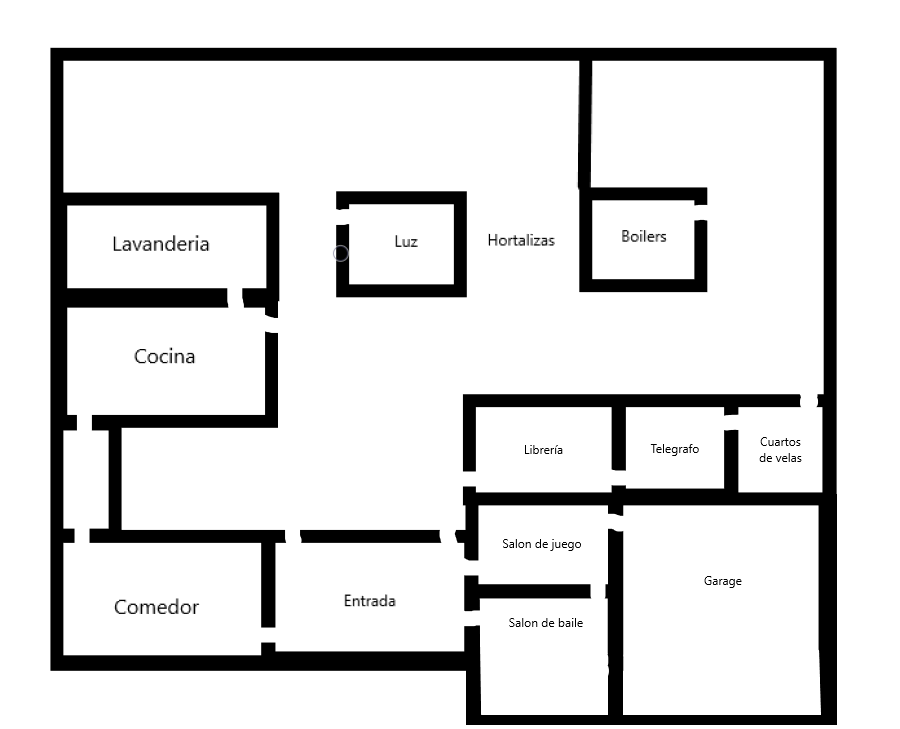
\includegraphics[width=1\linewidth]{images/MapaJuego.png}
    \caption{Organización del mapa del juego}
    \label{fig:mapa_juego}
\end{figure}
El juego se lleva a cabo en una mansión. El mapa consiste en un solo piso. Algunas de las características que se consideró que tuviera el mapa fueron:
\begin{itemize}
    \item Interconectado para permitir a los programadores moverse a completar sus actividades, de preferencia más de una salida entre cuartos. 
    \item Hay algunos cuartos que rompen con la primera regla para los programadores, tienen una sola salida y es muy fácil de que un asesino agarre a un programador haciendo una tarea y fácilmente lo pueda matar. Dado que hay poco flujo de tránsito, la tumba puede quedar no detectada por un rato. La forma de balancear esto es agregando varias tareas en este cuarto de forma que otros jugadores tengan la necesidad de entrar. Algunos jugadores más experimentados dada la reputación de esos cuartos podrán entrar a revisar si no hay ninguna tumba de alguno de sus compañeros programadores.
    \item Áreas grandes principales donde los jugadores circulan a las diferentes salas del juego, normalmente son zonas que un asesino consideraría muy alto riesgo para matar a un programador. Estas son la entrada a la mansión, un patio, el zaguán de atrás de la casa y un patio que conecta los \textit{boilers} con un corral.
\end{itemize}

El diseño del mapa se puede ver en la figura~\ref{fig:mapa_juego}.

\section{Desarrollo}
Usando las libertades dadas por la librería Mirror, se usó el mismo proyecto de Unity para el desarrollo del cliente y el servidor, usando el lenguaje de programación C\#. El servidor se encarga de hospedar las partidas y los clientes que dependen del servidor para manejar el estado. En el fondo la librería se encarga de sincronizar estado además de realizar llamadas y ejecutar funciones RPC a petición del servidor.

El juego se diseñó con un servidor autoritativo, algunos sistemas hacen cálculos en el servidor o las decisiones son rectificadas en este. En sí, el estado del juego será computado mayormente en el servidor, donde el cliente solo estará como un cliente ligero. La comunicación entre estos dos se realizara con el protocolo usando \textit{Websockets} para la transferencia de información, una limitación dada por el soporte de protocolos de comunicación del navegador web.

En esta etapa se realizó la programación de diversos sistemas y comportamientos de distintos elementos del juego.

\subsection{Creación de \textit{sprites} y \textit{assets}}
Según detalles del documento de diseño, se crean los diversos sprites para personajes, animaciones, objetos (mesas, cajas) e interfaces gráficas. Se crearon de todo aquello que no se pudo obtener de spritesheets de uso libre o porque fueron originales para este juego (se hablará de esto más adelante). El diseño de algunos artículos originales se realizó previamente en el documento de diseño del juego. Para los \textit{sprites} se definieron algunas limitantes, como la resolución, donde cada \textit{tile}  tiene medidas de 16x16, el fondo de este es transparente. En los \textit{sprites} necesarios, estuvieron los de personajes jugables (figura~\ref{fig:sprite_johanna}. Estos se diseñaron en \textit{Photoshop}. En el caso de los jugadores miden 1x2 \textit{tiles}. Las mesas (comedor, mesa de billar) son 3x3 \textit{tiles}. 

\begin{wrapfigure}{r}{0.25\textwidth}
    \centering
    
\includegraphics[width=0.25\linewidth]{images/JohannaOrdonez.png}
    \caption{Sprite de uno de los personajes jugables}
    \label{fig:sprite_johanna}
\end{wrapfigure}

Se encontraron \textit{spritesheets} que se pudieran usar con licencia en el proyecto en el sitio web \url{http://itch.io}, esto permitió reducir el trabajo de crear arte para el juego.
Entre estos fueron:
\begin{itemize}
    \item \textbf{Grass++} Variedad de sprites de pastos, flores y misceláneos para los patios y jardines
    \item Platformer 2D Tileset
    \item Dungeon Tileset
    \item Free Tileset Objects - Treasure Chests
\end{itemize}

\subsection{Puzzles}
        \begin{figure}[H]
        \centering
        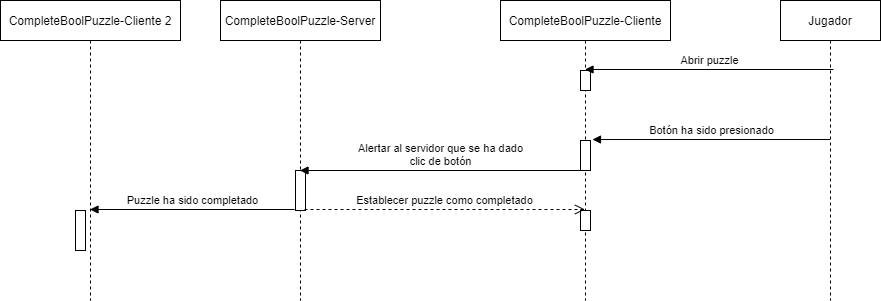
\includegraphics[width=0.8\linewidth]{images/DiagramaSecuenciaPuzzleBool.png}
        \caption{Diagrama de secuencia puzzle de encender generador (booleanos y comando si entonces)}
        \label{fig:diagrama_sec_booleano}
    \end{figure}
        \begin{figure}[H]
        \centering
        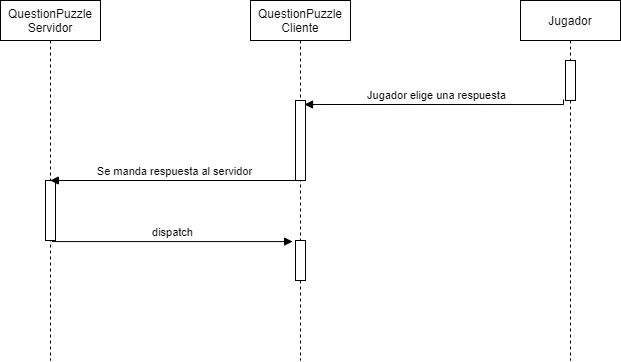
\includegraphics[width=0.8\linewidth]{images/DiagramaSecuenciaPuzzleSecuencia.drawio.png}
        \caption{Diagrama de secuencia del puzzle de secuencia }
        \label{fig:diagrama_sec_sec}
    \end{figure}
        \begin{figure}[H]
        \centering
        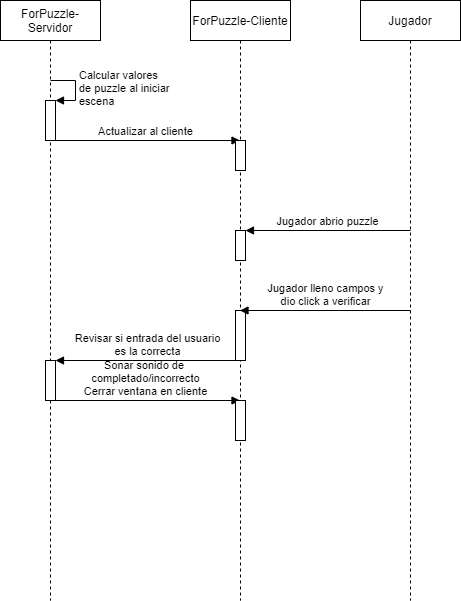
\includegraphics[width=0.4\linewidth]{images/diagrama_sec_for_while.png}
        \caption{Diagrama de secuencia puzzle completar ciclos}
        \label{fig:diagrama_sec_for_while}
    \end{figure}
        \begin{figure}[H]
        \centering
        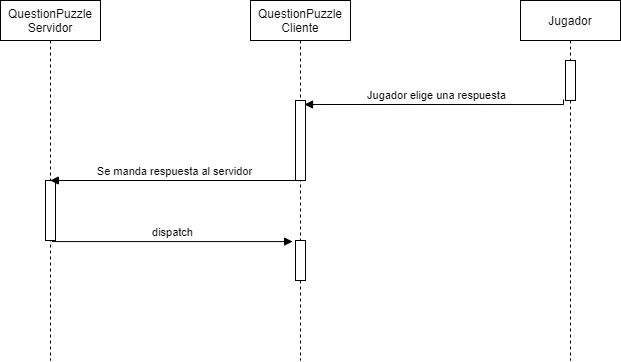
\includegraphics[width=0.8\linewidth]{images/DiagramaSecuenciaPuzzleOpcionMultiple.png}
        \caption{Diagrama de secuencia del sistema para puzzles de opción múltiple}
        \label{fig:diagrama_sec_opmul}
    \end{figure}
        \begin{figure}[H]
        \centering
        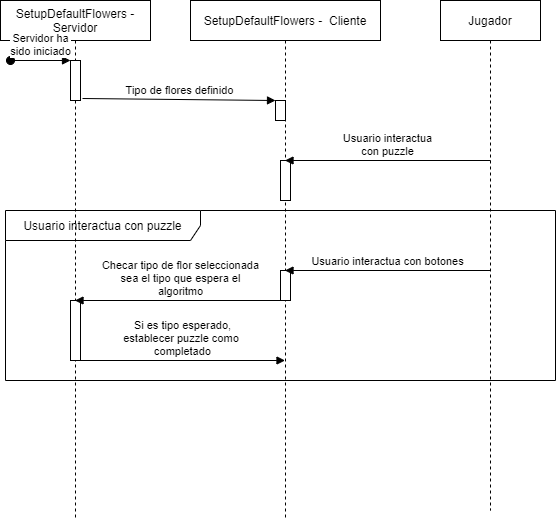
\includegraphics[width=0.8\linewidth]{images/DiagramaSecuenciaPuzzleIf.png}
        \caption{Diagrama de secuencia puzzle if}
        \label{fig:diagrama_sec_if}
    \end{figure}
        \begin{figure}[H]
        \centering
        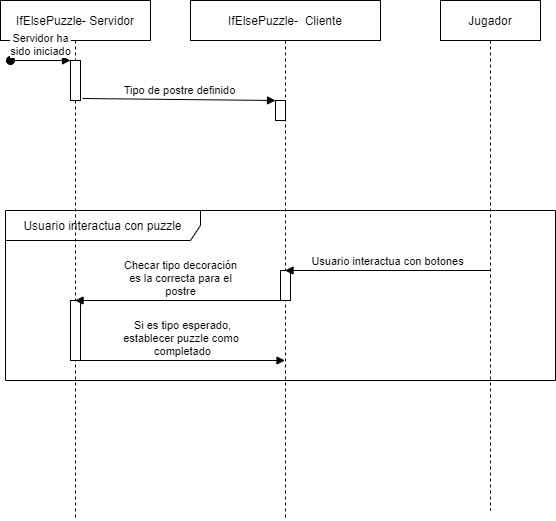
\includegraphics[width=0.8\linewidth]{images/DiagramaSecuenciaPuzzleIfElse.png}
        \caption{Diagrama de secuencia puzzle if else}
        \label{fig:diagrama_sec_if_else}
    \end{figure}
\begin{itemize}
    \item Completar ciclos: Los \textit{puzzle} de este tipo tienen varios campos a completar como se ha hablado anteriormente. Al llenar estos campos, el jugador tiene un botón de verificar, esto manda las entradas a través de la red al servidor, donde se verifica en el servidor. Ya sea respuesta correcta o falsa se comunica el resultado al cliente (figura~\ref{fig:diagrama_sec_for_while}).
    \item Secuencia: Los puzzle de secuencia usan una tabla simulada aprovechando los componentes de \textit{layout} provistos por Unity para el sistema de UI. Se creo un \textit{prefab} para poderlo \textit{spawnear} suficientes cuadritos para el tamaño del campo de juego establecido para el \textit{puzzle}. \texttt{SequenceGrid} es la clase que controla en comportamiento del \textit{puzzle} en el cliente, esta hace la labor de actualizar \textit{sprites} del \textit{grid} cuando hay cambios de posición del jugador. Todos estos subsistemas son controlados por SequencePuzzle que se encarga de leer las instrucciones en el cliente. Al terminar de leer las instrucciones, se mandan al servidor para verificar que lleguen a la meta (y marcar el \textit{puzzle} como completado) y en el cliente hacer un \textit{replay}, es visualmente atractivo, permite al jugador ver donde se equivocó y da continuidad al jugador que completo correctamente la tarea en lugar de marcar como completado el \textit{puzzle} automáticamente.
    \item  \textit{Puzzle} en área de generador (comando si/entonces y operadores relacionales): Este \textit{puzzle} incluye expresiones lógicas una dentro de la otra, los jugadores tendrán que analizar cómo se comporta y a base del estado actual de las variables, elegir que rama eligió el programa (el comando si/entonces) como se ve en la figura~\ref{fig:diagrama_sec_booleano}.
    \item Elegir la opción correcta: Usado para algunos \textit{puzzles} de ciclos, hay distintos botones con opciones. El jugador da clic a la opción correcta. El juego manda el índice de la respuesta al servidor, si el índice está marcado como respuesta correcta entonces se marca como contestada correctamente (figura~\ref{fig:diagrama_sec_opmul}).
    \item If: En este puzzle, se agarra un \textit{enum} aleatorio de los posibles tipos de flores. Este tipo de flor será seleccionada para completar un pedazo de pseudocódigo. Aparte, se selecciona otro tipo de flor, de la misma manera, esta se ajusta en cuadro de imagen. Este puzzle consiste en preguntarle al jugador que hace el seudocódigo dado el tipo de flor que pide y el tipo flor que va a procesar. La respuesta seleccionada se manda al servidor (figura~\ref{fig:diagrama_sec_if}).
    \item If/else: El \textit{puzzle if/else} necesita un valor booleano que se calcula cuando inicia el servidor, este valor es usado para decidir si se va a decorar un pastel o un \textit{cupcake}, como se había visto anteriormente le mostramos al jugador un pseudocódigo de la forma que debería de decorar el postre. Y el jugador manda al servidor su elección usando los dos botones para seleccionar, que se revisa que sea el valor correcto en el servidor como se nota en la figura~\ref{fig:diagrama_sec_if_else}.
\end{itemize}


\subsection{Sistema de versiones}
Para la elaboración del proyecto se usó el sistema de versiones Git. El repositorio es público y puede ser accedido en \url{https://github.com/SaulNunez/Project-Hamilton}.

\subsection{Integración Continua}
Se usó Github Actions permite ejecutar archivo de definición de tareas después de crear nuevos \textit{commits}.
Este ejecuta las siguientes acciones cada vez que se activa el trabajo:
\begin{itemize}
    \item Compila ejecutables para Linux x64-86 y WebGL
    \item Corre las pruebas unitarias del proyecto (no se desarrollo ninguna por cuestiones de tiempo, pero la tarea esta habilitada y funcionando) 
    \item Crea documentación de las funciones y variables del proyecto y sube a \textit{Github Pages} la nueva versión, esta es accesible en la página  \url{http://saulnunez.com/Project-Hamilton/}
\end{itemize}

Para la compilación de ejecutables y el sistema pruebas se usó el increíble trabajo de GameCI que tiene imágenes preconfiguradas de Unity que facilitan la creación de los \textit{pipelines} necesarios. Se uso su tutorial disponible en \url{https://game.ci/docs/github/v1/builder} y sus ejemplos para la creación del archivo de configuración.

En la creación del pipeline de la generación de documentación se usó el trabajo de Normand Erwan disponible en \url{https://github.com/NormandErwan/DocFxForUnity} que provee la configuración de DocFX para que funcione con la organización por carpetas de Unity y por la forma en la que este de manera predefinida crea clases para componentes en el \textit{namespace} \textbf{global}.

\section{Implementación}
\subsection{Sprites}
Como lo vimos anteriormente, hay dos tipos de \textit{sprites}. Aquellos que se obtuvieron de itch.io se agregaron simplemente a Unity importándolos a las carpetas del proyecto y configurado para que los interpretara como \textit{"sprites"}, estos al ser \textit{spritesheets} (y por lo tanto contener en un solo archivo un numero de \textit{sprites} individuales) se cortan en el editor de \textit{sprites} dependiendo del tamaño en el que fueron diseñados (normalmente 16x16 o 32x32 píxeles); normalmente aquí acabaría el proceso pero en algunos sprites requirieron ajustes manuales por su forma de \textit{"sprite packing"} (como se organizan los sprites entre el archivo de imagen). En el segundo tipo, fueron los creados específicamente para el juego, estos fueron diseñados en Photoshop, se usó el \textit{plugin} de PSDs para permitir importar archivos de Photoshop directamente a Unity para utilizarlos, dependiendo de la situación del \textit{sprite} en particular se dejaba en simple o en múltiples, estos últimos cortados en  16x16 para ítem grandes que usan el principio 9-slice.

\subsection{Emergencias}
\begin{figure}[h]
    \centering
    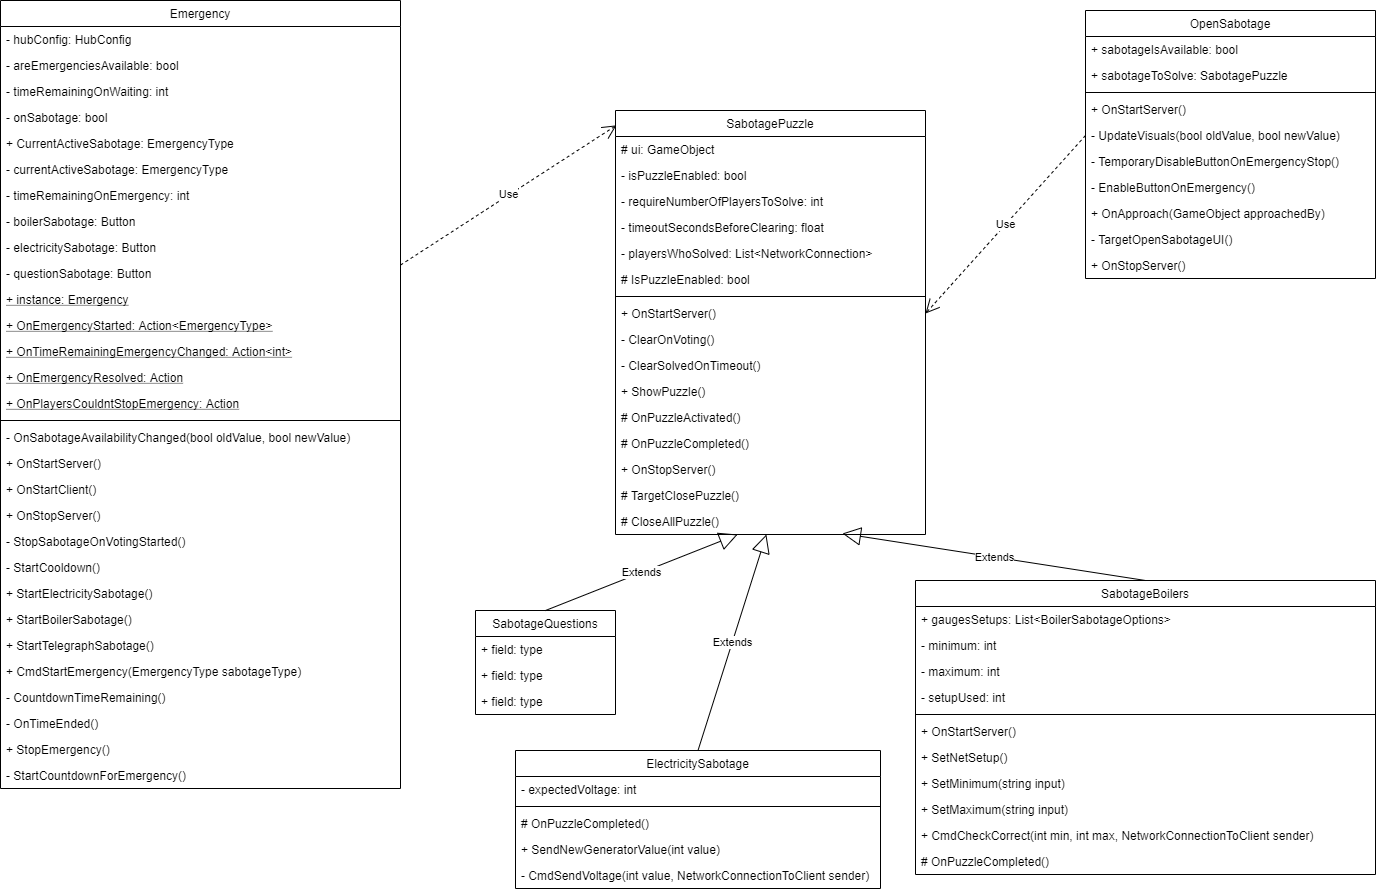
\includegraphics[width=1\linewidth]{images/DiagramaClasesEmergencias.png}
    \caption{Diagrama de clases del sistema de emergencias}
    \label{fig:diagrama_clases_emergencias}
\end{figure}
\begin{figure}[p]
            \centering
            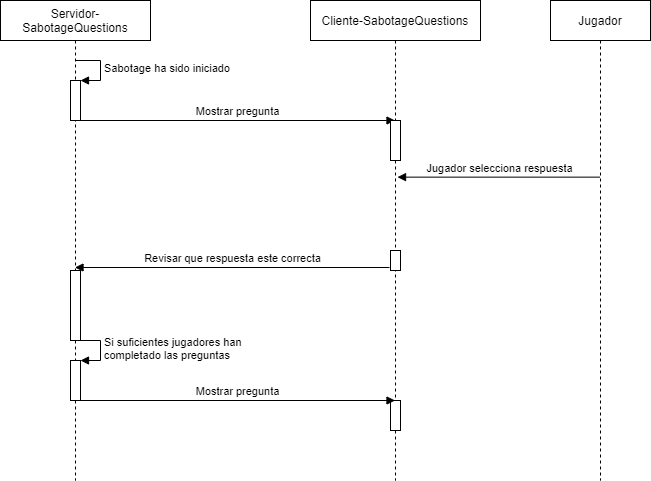
\includegraphics[width=1\linewidth]{images/diagrama_secuencia_sabotage_preguntas.png}
            \caption{Diagrama de secuencia de emergencia de telégrafo}
            \label{fig:diagrama_secuencia_emergencia_pregunta}
        \end{figure}
        \begin{figure}[p]
            \centering
            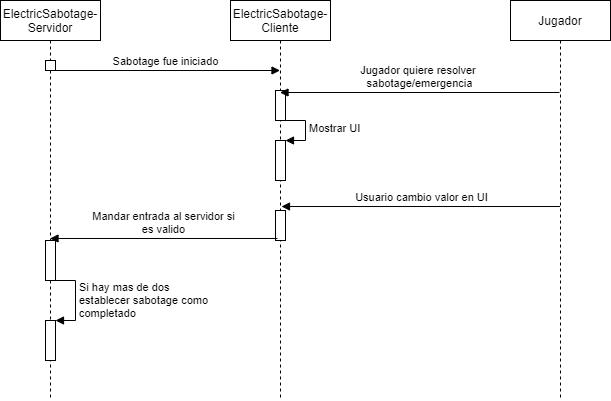
\includegraphics[width=1\linewidth]{images/DiagramaSecuenciaSabotageGeneradores.png}
            \caption{Diagrama de secuencia de emergencia en los generadores}
            \label{fig:diagrama_secuencia_generadores}
        \end{figure}
Para las emergencias se decidió crear un subsistema para controlar su estado. Este controla la interfaz que tienen los impostores para encender las emergencias. Así como los \textit{timeouts} necesarios para que las emergencias tarden un tiempo determinado antes de poder ser activados cuando inicia el juego y cuando se reinicia el contador por una votación para sacar a alguien o por el \textit{cooldown} a una emergencia previa.
Como los emergencias incluyen acciones comunes como activarlos o detenerlos, se creó una clase base que usan todos estos para incluir estos métodos (figura~\ref{fig:diagrama_clases_emergencias}).
\begin{itemize}
    \item Emergencia de telégrafo, la selección de pregunta y su revisión ocurren en el servidor, el cliente recibe información sobre la pregunta actual (para mostrarla en pantalla) y todo mundo(como todos los que están respondiendo el emergencia, mínimo los dos jugadores) tiene que contestar la pregunta actual para poder pasar a la siguiente, como se ve en la figura~\ref{fig:diagrama_secuencia_emergencia_pregunta}.
    \item Apagar generadores, la única función que realiza el cliente es mandar la nueva posición del \textit{slider} al servidor, como se puede ver en la figura~\ref{fig:diagrama_secuencia_generadores}.
    \item Ajustar presión del boiler, hay distintos medidores de los cuales elige uno para mostrar por emergencia, al definirse uno, se actualiza la UI en el cliente, cada vez que el jugador juegue con los valores del algoritmo que el usuario necesita completar para regular la presión se revisara en el cliente que son el valor ideal.
\end{itemize}

\subsection{Despliegue}
\begin{figure}[H]
    \centering
    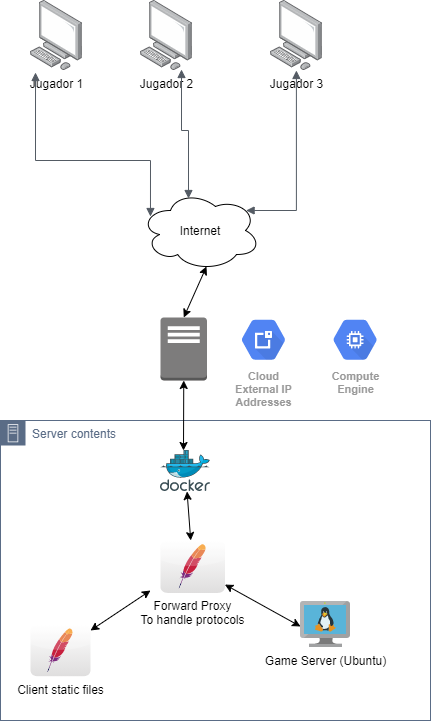
\includegraphics[width=0.5\linewidth]{images/diagrama_deployment.png}
    \caption{Diagrama del despliegue, en este caso un servidor en \textit{Google Cloud Compute Engine}}
    \label{fig:diagrama_despliege}
\end{figure}
Se crearon dos imágenes de \textit{Docker} para hospedar los programas del  servidor y un \textit{webserver} usando Apache para servir la página del juego para los cliente. Estos contenedores pueden ser manejados por \textit{Docker Compose} para controla su estado y crea una red local simulada entre estos, en el proyecto se creo el archivo llamado \textbf{docker-compose.yml} que orquestra estos contenedores detallados y adicionalmente un tercero que va enfrente de los anteriormente detallados para servir como \textit{forward proxy}, que distribuye los paquetes según su protocolo (\textit{HTTP} a \textit{webserver} y \textit{websockets} al servidor), este ultimo utiliza Apache. La función de este \textit{forward proxy} es poder dirigir todas las peticiones a ambos contenedores por el puerto 80, para evitar cualquier bloqueo por \textit{firewalls}. El diagrama de la conexión entre los contenedores y el mundo real se puede ver en la figura~\ref{fig:diagrama_despliege} en un ejemplo en el que esta hospedado en \textit{Google Cloud Compute Engine}, el \textit{stack} de red del servidor manda los paquetes de red a Docker que a la vez la delega a los contenedores.
En el caso específico del cliente que corre cada usuario se usó Apache para el \textit{host} de los archivos estáticos.
Para el contenedor del servidor se uso como imagen base \textit{Ubuntu}, en el que se llevó a cabo la configuración según las guía de \textit{Mirror networking} donde lo hospedan en \textit{Google Cloud}, esta disponible en: \url{https://mirror-networking.gitbook.io/docs/guides/server-hosting/google-cloud}, cabe destacar que la imagen de Ubuntu para Docker no trae los paquetes para X11, 

Se creó documentación para montarlo en otros servidores, esta disponible en el archivo \textbf{README.md} en la raíz del repositorio del proyecto.

\section{Pruebas}
Durante el desarrollo se usaron pruebas de humo en el producto, se usó el \textit{asset} \href{https://github.com/hwaet/UnityProjectCloner}{UnityProjectCloner} para crear una copia del proyecto para poder simular en la misma computadora un cliente y lo que la librería Mirror llama un \textit{host}, un cliente con el servidor integrado, a base de esto poder probar que el código generado tenía el funcionamiento esperado y que no tuviera errores o problemas de configuración. Fueron pruebas de 5-15 minutos sobre el sistema que se estaba trabajando en ese momento.

Se hicieron tres \textit{soak tests} distintos. Uno se dejó durante 3 horas la pantalla de inicio, en el segundo se dejó el \textit{lobby} y en la tercera una sesión del juego.

Se hicieron pruebas de funcionalidad en una ocasión, con 3 jugadores para revisar la usabilidad de la interfaz gráfica, ver la estabilidad y ver problemas en las mecánicas del juego.

Adicionalmente se realizó una sesión donde se simulo una partida con tres jugadores para hacer pruebas del multijugador con un servidor remoto para ver si ocurrían problemas debido a la latencia entre el cliente y el servidor debido a la distancia de la conexión con el servidor.
